%% This is file `elsarticle-template-1-num.tex',
%%
%% Copyright 2009 Elsevier Ltd
%%
%% This file is part of the 'Elsarticle Bundle'.
%% ---------------------------------------------
%%
%% It may be distributed under the conditions of the LaTeX Project Public
%% License, either version 1.2 of this license or (at your option) any
%% later version.  The latest version of this license is in
%%    http://www.latex-project.org/lppl.txt
%% and version 1.2 or later is part of all distributions of LaTeX
%% version 1999/12/01 or later.
%%
%% Template article for Elsevier's document class `elsarticle'
%% with numbered style bibliographic references
%%
%% $Id: elsarticle-template-1-num.tex 149 2009-10-08 05:01:15Z rishi $
%% $URL: http://lenova.river-valley.com/svn/elsbst/trunk/elsarticle-template-1-num.tex $
%%
\documentclass[preprint,12pt,authoryear]{elsarticle}

%Prevents that citations cross the margin of the manuscript
\usepackage{breakcites}

%Bold Greek letters
\usepackage{bm}

%% Use the option review to obtain double line spacing
%% \documentclass[preprint,review,12pt]{elsarticle}
%% Useful packages
\usepackage{amsmath}
\usepackage[colorinlistoftodos]{todonotes}
\usepackage[colorlinks=true, allcolors=blue]{hyperref}

\usepackage{hyperref}
%\usepackage[autostyle]{csquotes}

%%Floatbarrier prevents figures to be above section title 
\usepackage{placeins}

\usepackage{array}
\newcolumntype{P}[1]{>{\centering\arraybackslash}p{#1}}

%% Use the options 1p,twocolumn; 3p; 3p,twocolumn; 5p; or 5p,twocolumn
%% for a journal layout:
%% \documentclass[final,1p,times]{elsarticle}
%% \documentclass[final,1p,times,twocolumn]{elsarticle}
%% \documentclass[final,3p,times]{elsarticle}
%% \documentclass[final,3p,times,twocolumn]{elsarticle}
%% \documentclass[final,5p,times]{elsarticle}
%% \documentclass[final,5p,times,twocolumn]{elsarticle}

%% The graphicx package provides the includegraphics command.
\usepackage{graphicx}
%% The amssymb package provides various useful mathematical symbols

%%Allows text in equations
\usepackage{amssymb}
%%Make sure caption does not stick to the table
\usepackage{caption} \captionsetup[table]{skip=10pt}
%%Multiple rows in complex tables
\usepackage{multirow}

%%Two figures aside
\usepackage{caption}
\usepackage{subcaption}

%%Forced line break within cell
\usepackage{makecell}
\renewcommand\theadalign{bc}
\renewcommand\theadfont{\bfseries}
\renewcommand\theadgape{\Gape[4pt]}
\renewcommand\cellgape{\Gape[4pt]}

%% The amsthm package provides extended theorem environments
%% \usepackage{amsthm}

\usepackage[T1]{fontenc}
\usepackage[utf8]{inputenc}
\usepackage{floatrow}

%Packages for running title
\usepackage{fancyhdr}
\pagestyle{fancy}

%% The lineno packages adds line numbers. Start line numbering with
%% \begin{linenumbers}, end it with \end{linenumbers}. Or switch it on
%% for the whole article with \linenumbers after \end{frontmatter}.
\usepackage{lineno}

%% Double space
\usepackage{setspace}

%Acknowledgements
\newcommand{\ackname}{Acknowledgements}

%Authors’ contributions
\newcommand{\autcont}{Authors’ contributions}

%Data accessibility 
\newcommand{\datacc}{Data accessibility}

\usepackage{moreverb} % for verbatim output

%% natbib.sty is loaded by default. However, natbib options can be
%% provided with \biboptions{...} command. Following options are
%% valid:

%%   round  -  round parentheses are used (default)
%%   square -  square brackets are used   [option]
%%   curly  -  curly braces are used      {option}
%%   angle  -  angle brackets are used    <option>
%%   semicolon  -  multiple citations separated by semi-colon
%%   colon  - same as semicolon, an earlier confusion
%%   comma  -  separated by comma
%%   numbers-  selects numerical citations
%%   super  -  numerical citations as superscripts
%%   sort   -  sorts multiple citations according to order in ref. list
%%   sort&compress   -  like sort, but also compresses numerical citations
%%   compress - compresses without sorting
%%
%% \biboptions{comma,round}

% \biboptions{}

% Glossary
\usepackage[utf8]{inputenc}
\usepackage{hyperref}
\usepackage{glossaries}
\usepackage{calc}
\usepackage{booktabs}
\usepackage{tabularx}% (for comparison)

\journal{Ecological Modelling}

% Running title
\rhead{Decision-making models for passive telemetry data}
\lhead{}

\begin{document}

%double spacing to facilitate the reviewing process
\doublespacing

\begin{frontmatter}

%% Title, authors and addresses

\title{Combining disciplines: dealing with observed and cryptic animal residencies in passive telemetry data by applying econometric decision-making models  \\
}

%% use the tnoteref command within \title for footnotes;
%% use the tnotetext command for the associated footnote;
%% use the fnref command within \author or \address for footnotes;
%% use the fntext command for the associated footnote;
%% use the corref command within \author for corresponding author footnotes;
%% use the cortext command for the associated footnote;
%% use the ead command for the email address,
%% and the form \ead[url] for the home page:
%%
%% \title{Title\tnoteref{label1}}
%% \tnotetext[label1]{}
%% \author{Name\corref{cor1}\fnref{label2}}
%% \ead{email address}
%% \ead[url]{home page}
%% \fntext[label2]{}
%% \cortext[cor1]{}
%% \address{Address\fnref{label3}}
%% \fntext[label3]{}


%% use optional labels to link authors explicitly to addresses:
%% \author[label1,label2]{<author name>}
%% \address[label1]{<address>}
%% \address[label2]{<address>}

\author{Stijn Bruneel$^{1,2\ast}$, Pieterjan Verhelst$^{2}$, Jan Reubens$^{3}$, Stijn Luca$^{4}$, Johan Coeck$^{5}$, Tom Moens$^{2}$, Peter Goethals$^{1}$}

\address{$^{1}$Department of Animal Sciences and Aquatic Ecology, Ghent University, Coupure Links 653, 9000 Ghent, Belgium,

$^{2}$Marine Biology Research Group, Ghent University, Krijgslaan 281, 9000 Ghent, Belgium,

$^{3}$Flanders Marine Institute (VLIZ), Wandelaarkaai 7, 8400 Ostend, Belgium,

$^{4}$Department of Data Analysis and Mathematical Modelling, Ghent University, Coupure Links 653, 9000 Ghent, Belgium,

$^{5}$Research Institute for Nature and Forest (INBO), Havenlaan 88, bus 73, 1000 Brussels, Belgium,

$^\ast$To whom correspondence should be addressed; E-mail: stijn.bruneel@ugent.be}

\begin{abstract}
% Text of abstract

% \begin{minipage}[t]{0.9\linewidth}
% \end{minipage}
% \vtop{%
%   \vskip-1ex
%   \hbox{%
%     \includegraphics[width=0.9\linewidth]{Figures/GraphicalAbstract}%
%   }%
% }%

% \clearpage

Migratory species do not necessarily behave migratory continuously. An important aspect of studying migratory species is therefore to distinguish between movement and resident behaviour. Telemetry is a rapidly evolving technique to study animal movement, but the number of data processing techniques to account for resident behaviour remains limited. In this study we describe how models that were initially developed to predict human customer behavior, i.e. two-part and three-part models, provide new insights in the movement of migrating eel by accounting for resident behaviour apparent from telemetry data sets. In econometrics, two-part models take into account that the decision of a customer to purchase an item and the decision of the customer on the purchase quantity of the concerning product, might be affected by different factors. Similarly, the factors that affect the decision of a fish to migrate or to stay resident might be different from the factors that affect the swimming speed of the fish. Telemetry data of eel movement in the Permanent Belgian Acoustic Receiver Network (PBARN) of the Scheldt Estuary was used. This network with high detection probabilities allowed residencies to be recognized, defined, and introduced as zero values in a movement-residency data set. Two-part models, which consider movement decision, i.e. residency or movement, and movement intensity, i.e. swimming speed, as two different processes or parts of one larger model, outperformed one-part models that do not make that distinction. This underlines the complex migration behaviour eels exhibit. These two-part models in turn were outperformed by three-part models that also accounted for cryptic (i.e. unobserved) residencies. While the one-part model identified the tides and the distance from the most upstream gate as most important for movement, the three-part models identified the tides as most important for the movement decision and the distance from the most upstream gate as most important for the movement intensity. Considering movement decisions, cryptic residencies and movement intensity in modelling efforts increased model performance by 10 \%, underlining the importance of acknowledging the potentially complex behaviour animals exhibit. 

\end{abstract}

\begin{keyword}
Acoustic telemetry \sep Fish movement \sep Residency \sep Gate \sep Two-part and three-part model \sep Eel migration

%% keywords here, in the form: keyword \sep keyword

\end{keyword}

\end{frontmatter}

%%
%% Start line numbering here if you want
%%
\linenumbers

%% main text
\section{Introduction}
\label{Introduction}

Zero values are often encountered in ecological count data where they typically represent absences. However, zeros may have different meanings as they may arise from real absences due to habitat unsuitability, or from false absences due to observer and design errors \citep{Blasco-Moreno2019WhatEcology}. Similarly, in telemetry studies, data-sets can be heavily zero-inflated if moments of non-detection are considered as zeros \citep{Brownscombe2019ConductingManagers,Whoriskey2019CurrentDetections}, with the meaningfulness of these zeros being strongly dependent on the network design \citep{Bruneel2020QuantifyingSystems}.
Since the objective of many telemetry studies is to describe movement behaviour of animals, zero values could be used as an indication of non-movement or residency. However, accounting for resident behavior, represented as zero values in telemetry data, might require adapted models. Therefore, the aim of this study is to evaluate currently used models and to assess the potential of alternative models to deal with such data. 

A good network design is key to defining zero values. In estuarine and riverine acoustic networks with good detection probabilities, receivers may act as gates that tagged animals need to pass to leave a specific area \citep{Kraus2018,Steckenreuter2017}. Therefore, animals which remain undetected could still be positioned within a zone of the study area, i.e. between two gates, allowing periods of non-detection to be considered as residencies between detections \citep{Bruneel2020QuantifyingSystems}. 

However, the specific animal behaviour between detections often remains entirely unknown, unless some expert-knowledge, such as typical swimming speed and spawning period, is integrated. For example, a fish known to migrate during a certain period would be expected to perform highly unidirectional movement behavior and unexpected travel delays would be an indirect indication of resident behavior between detections. Since these residencies between detections cannot be observed directly, they are referred to as cryptic residencies. 

Zero-inflated data sets often require adapted statistical tools. Depending on the nature of zeros, different statistical ecological models have been suggested. If both false and true zeros are likely to be present, zero inflated models are typically used, while hurdle models are used when there are only true zeros \citep{Zuur2009}. More specifically, hurdle models assume that two processes result in two distinct signals, i.e. zero versus not zero, while zero-inflated models assume that both processes can yield zero values. For example, in case detection probabilities are low, individual fish not being detected might actually be present, yielding false zeros in addition to structural zeros. In such a case, zero-inflated models would be most appropriate. Within the field of ecology, zero-inflated and hurdle models are typically used for modelling count data inflated with observed absences \citep{Blasco-Moreno2019WhatEcology,Joseph2009ModelingMechanisms,Zuur2009}. Although continuous and proportional ecological data sets are omnipresent, model equivalents for these types of data are not often used. However, for continuous ecological data, such as fish swimming speed, models with a similar approach but different underlying distribution could be useful (i.e. while for count data, Poisson or negative binomial distributions are typically used, Gaussian or Gamma distributions would be more appropriate for continuous data). In econometric studies for example, the continuous equivalents of hurdle models, known as two-part models, have already been used frequently \citep{Deb2002EstimatesModels,Farewell2017Two-PartData}. 

Excess zeros are often considered a nuisance as they typically require more complex models with more parameters to be defined \citep{Warton2005ManyData}. However, explicitly accounting for zero-values may be useful as they may represent a unique signal of an unconsidered process. For example, in econometrics, two-part models have been widely used to study customer behaviour \citep{Neelon2016ModelingOverview,Pohlmeier1995AnHealthcare}. A customer might decide to purchase a product (Will I buy this?), but after that decision he/she would also need to decide on the quantity of the product (How much of it will I buy?). The conditions that drive the customer to purchase may be different from those driving the level of consumption. Hence, accounting for each process separately may be necessary to understand customer behavior.

Similarly, the factors that trigger fish movement, i.e. the movement decision, may be different from the factors determining the distance or speed with which the fish moves, i.e. the movement intensity. Hence, accounting for movement decision and intensity separately may also be necessary to understand fish movement behavior. Therefore, the aim of this study was to assess the added value for predictions and the implications for ecological knowledge of distinguishing between both processes of fish movement behavior. More specifically, we compared the predictive performance and inferred ecological knowledge of one-part and two-part models describing the movement behaviour of migrating eel (\textit{Anguilla anguilla L.}) in the Scheldt Estuary. In addition, to assess whether a further compartmentalization (e.g. distinction between upstream and downstream movement) would provide added value, different three-part models were constructed and compared with the one-part and two-part models. 

Given the increasing data availability and complexity entailed by the exponential increase of possible associations among predictors, machine learning is gaining ground among movement ecologists because of its high predictive performance and alleged ease of use \citep{Joseph2017ApplicationsStudies,Wang2019MachineData}. However, although machine learning is built on a statistical framework, the outputs of pattern-learning algorithms are often difficult to interpret in the wider context of system functioning \citep{Bzdok2018PointsLearning}. Therefore, in practice, the choice between machine learning and statistical models is typically determined by the purpose, which is either to make predictions or to infer knowledge, respectively. However, since ecologists typically want the best of both worlds, i.e. a model that is interpretable in terms of ecological knowledge while remaining broadly applicable for predictions, statistical models and machine learning should be treated as complementary tools. Therefore, we also compared the interpretability and the predictive performance of statistical models (i.e. one-part and two-part regression models), hybrid models (i.e. three-part models that combine neural networks with generalized linear regression) and machine learning algorithms (i.e. conditional inference random forests (RF)) for the current telemetry data set.

\section{Materials and methods}

\subsection{Study area}

The Schelde Estuary is a well-mixed estuary of 160 km long without transversal man-made migration barriers and characterized by strong currents, high turbidity and a large tidal amplitude up to 6 m \citep{Cornet2016}. The estuary can be divided in two regions (upstream to downstream): the Zeeschelde, which spans 105 km from Ghent to Antwerp (Belgium), and the Westerschelde, which covers the 55 km from Antwerp to the mouth of the estuary at Vlissingen (The Netherlands). The width of the Zeeschelde varies between 50 to 1350 m while the width of the Westerschelde varies between 2000 and 8000 m (Fig. \ref{fig:network}). The description of the study area was adopted from \cite{Bruneel2020QuantifyingSystems}. This study was limited to the part of the Zeeschelde, because of the relatively low detection probability of the gates in the Westerschelde (see section \ref{acousticnetwork}). 

\subsection{Tagging procedure}

At the tidal weir in Merelbeke (Ghent), 100 eels were caught and internally tagged with V13 (VEMCO Ltd., Canada) coded acoustic transmitters \citep{Verhelst2018}. After capture, surgery and recovery \citep{Thorstad2013b}, fish were released at the nearest receiver. Of the 100 tagged eels, 58 migrated. The migration period of these 58 eels was determined \citep{Verhelst2018} and used for further analysis. A more detailed description of the tagging procedure is provided in \ref{Taggingprocedure}. The description of the tagging procedure was adopted from \cite{Bruneel2020QuantifyingSystems}.

\subsection{Acoustic network}
\label{acousticnetwork}

Within the framework of the Belgian LifeWatch observatory, a permanent longitudinal network of receivers (VR2W, VEMCO Ltd, Canada) has been deployed since the spring of 2014 in the Schelde Estuary \citep{Reubens2019TheNetwork}. Currently, the network consists of 25 receivers, deployed from the river bank, which were combined into 18 gates that are on average 4969 m apart (Fig. \ref{fig:network} and Table \ref{gate_list}). At four locations (s15, s16, s17 and s18), a receiver on each side of the estuary was deployed to cover the whole width. The exact detection range for the different receivers in the Zeeschelde was unknown, but ranges between 300 m and 1000 m \citep{Verhelst2018}. Results from the network in the North Sea suggest that it is strongly dependent on current velocity and wave action and will therefore be characterized by a strong spatial and temporal variability \citep{Reubens2018}. The detection probability of the gates was estimated using the conditional nature of fish movement throughout the system \citep{Brownscombe2019ConductingManagers}. Since there are no other pathways to the North Sea, tagged fish have to pass the different gates in a well-defined order and detection probability can be defined as the probability of detecting a tag moving past a specific gate \citep{Melnychuk2012,Perry2012UsingData}. The detection probabilities of the different gates are given in Table \ref{gate_list}. The description of the acoustic network was adopted from \cite{Bruneel2020QuantifyingSystems}. 

\begin{figure}[h!]
  \centering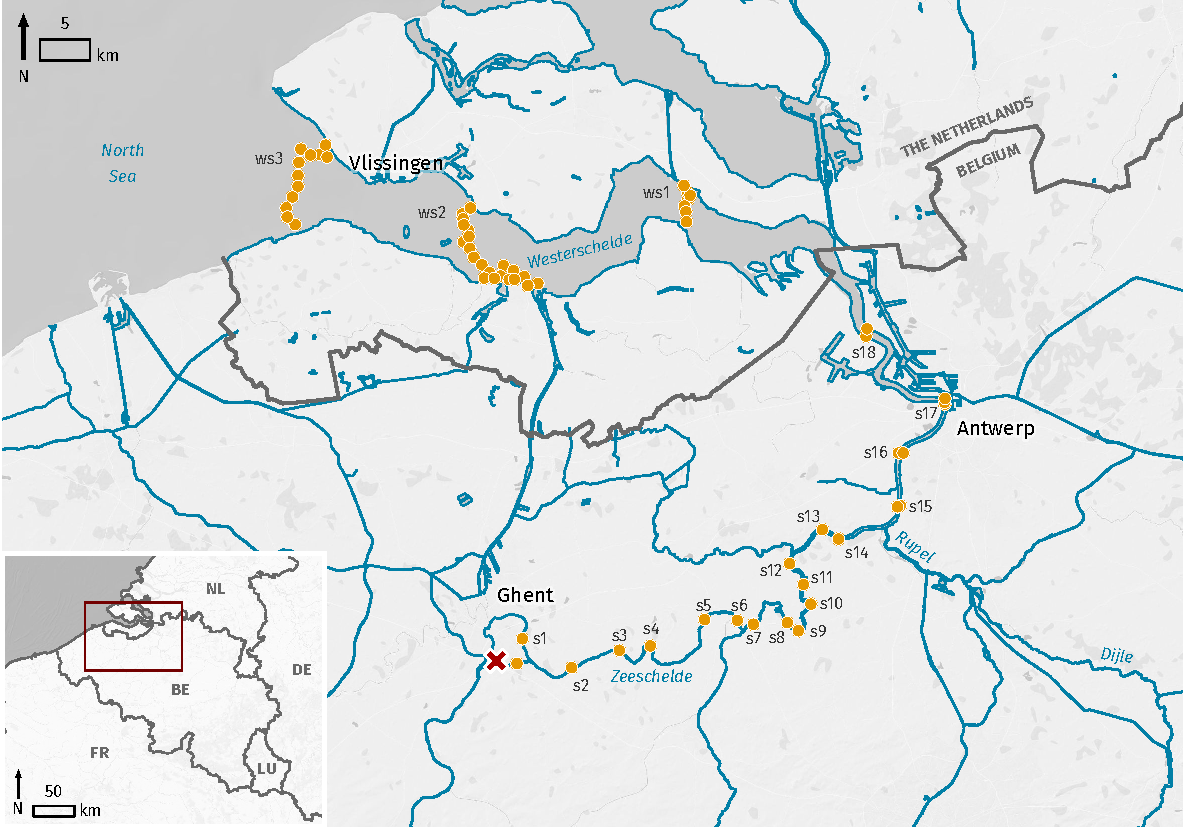
\includegraphics[scale=0.6]{receivernetwork-mechelen.pdf}
  \caption{The Schelde Estuary comprises the Zeeschelde (Ghent-Antwerp) and Westerschelde (Antwerp-Vlissingen). The receivers are represented as orange circles. The gates are indicated as labels for different groups of receivers. The weir in Ghent where the eels were caught and released is depicted as a red cross. Detections at the three gates in the Westerschelde (ws1, ws2 and ws3) were not considered in this study because of their relatively low detection probabilities. Adapted from \cite{Bruneel2020QuantifyingSystems}.}
  \label{fig:network}
\end{figure}

\subsection{Eel movement}

Given the high average detection probability of 97.0 \% in the Zeeschelde, the number of false zeros was likely limited. In addition, since the movement of eels is highly unidirectional once they have started migrating, eels not being detected at one gate are likely to be detected at the next gate, causing some reduction in resolution, but still providing a reliable position estimate. Since false zeros, due to low detection probabilities, are unlikely, we decided to work with two-part models instead of zero-inflated models.

When a tagged eel was consecutively detected at two different gates, we considered the time lapse between these two detections as a movement interval and the distance between the two gates was determined. When a tagged eel was detected multiple times at a specific gate without being detected at any other gate, the time lapse between the earliest and last detection was considered as a residency interval and was assigned a distance value of zero. It should be noted that some short intervals might actually have been identified incorrectly as residency intervals. For example, a migrating eel might come within the detection range and have multiple detections while moving from one side of the gate to the other. Although considered as highly variable in literature \citep{Breukelaar2009,Verbiest2012}, we assumed an average migration speed of 0.25 m s$^{-1}$ and a detection range of 250 meter, yielding an approximate threshold value of at least 30 minutes for residency intervals. To ensure that movement was not wrongly identified as residencies, this value was doubled and all residency intervals with a time span below 1 hour were omitted from the analysis (10.80 \% of the residency intervals were retained for analysis). 

It is possible that, before heading to the next gate, a tagged eel was resident between two gates without entering either gate's detection range. Such unobserved or cryptic residencies are not directly apparent from the data as  they are observed as being part of the movement interval. However, these cryptic residencies can be accounted for indirectly as they will cause a travel delay in the movement interval, negatively affecting the time necessary to reach the next gate.

Recognizing resident behavior in acoustic telemetry networks based on position estimates alone often remains a difficult objective \citep{Cagua2015}. In this specific study, indirect (i.e. through travel delays) and direct indications of apparent non-movement can be either the result of (i) fish choosing to be resident and to discontinue swimming or (ii) fish swimming against the currents without much net gain in distance covered. However, if there are clear signs of individual variation and enough individuals to account for it, a distinction between both can be made. When animals are resident, they cannot be distinguished from each other using position estimates alone. However, when they migrate, even against the current, the fastest individuals will reach higher swimming speeds and can as such be distinguished from slower individuals. It should be noted that throughout the manuscript, swimming speed represents the ground speed (i.e. geographical progress per unit of time) without correction for current speed. As each tag emits a signal at a unique frequency, individuals can be identified and individual variation in swimming speed can be determined and used to analyse the behavior associated with apparent non-movement. Since European eel and other migrating fish have been found to apply different strategies to save energy, it is much more likely that eels would choose the most energy efficient option and choose to be resident when facing currents rather than to swim without much net gain in distance covered \citep{Arnold1984FishShelf,Glebe1981Migration,Metcalfe1990TheSea}. Therefore, we consider measurements of apparent non-movement as residencies and evaluate afterwards whether this choice was justified based on the outcomes of the models.

To normalize the data, distances were divided by time, yielding swimming speed. Residency and movement intervals with a time lapse higher than one full tidal cycle were removed (13.42 \% data removal) as they do not allow to contribute movement behaviour to either ebb tide, flood tide or a combination of both (see section \ref{Environmental_data}). 
To account for telemetry detection errors that might cause unrealistic swimming speeds, movement intervals with a swimming speed  of 1.5 interquartile ranges (IQRs) below the first quartile or above the third quartile were considered outliers and removed from the data set \citep{Tukey1977ExploratoryAnalysis}. In practice, all movement intervals with a swimming speed higher than 2.7 or lower than -1.5 m/s were omitted from the analysis (additional 2.20 \% data removal). In summary, first 89.20 \% of residency intervals were removed, followed by a 13.42 \% removal from the entire data set (movement intervals + residency intervals), followed by a 2.20 \% removal from the entire data set. The final data set contained 19.24 and 80.76 \% residency and movement intervals, respectively. 

\subsection{Environmental data}
\label{Environmental_data}
As the biological response in this study was analysed at a relatively fine spatiotemporal resolution \citep{Bultel2014,Verhelst2018}, a sound coupling of biological and environmental data would have been challenging and use of daily averages would have yielded inconclusive results on within-day movement patterns. Therefore only variables were included that were fixed in time (i.e. distance from source), fixed in space (i.e. day phase), known to be accurate at high spatial and temporal resolutions (i.e. period of flooding and period of ebbing), or known to be well represented by daily averages (i.e. moon and tidal phase). It should be noted that the main aim of this study was to assess the potential of alternative ecological models rather than to identify all environmental factors affecting eel migration. To obtain a more comprehensive understanding of these environmental factors, more fine-scale measurements and/or simulations of potentially important environmental variables, such as discharge, temperature, salinity and precipitation could be used to fine-tune the developed models. 

The following description of the collection and processing of tidal data was adapted from \cite{Verhelst2018}: To account for the distances between the locations of the gates and of the tidal measuring stations (Hydraulic Information Centre, Belgium), a weighted average method was applied to estimate the precise moments of low and high water at the gates. The closest upstream and downstream tidal measuring stations were assigned to each gate. Based on the distances between these tidal stations and the gate, linear weights were assigned to both tidal stations. When tidal data at the respective upstream or downstream tidal station was absent or of questionable quality (e.g. outliers and known periods of malfunctioning measuring devices) at the time interval of interest, the next upstream or downstream tidal station was chosen. This allowed us to estimate the duration of ebbing and flooding for each movement and residency interval. 

The ratio of period flood tide (minutes) over total period of the interval (minutes) was determined and used as a predictor, i.e. flood ratio. Per gate, the ratio of the maximum difference in water level of the concerning day over the median of the maximum difference in water level per day of the entire study period was used as a proxy for tidal phase, with low values being associated with neap tide and large values with spring tide. Moon phase was a numerical value representing the degree of illumination of the moon, ranging from new moon (0) to full moon (1). Time of day was a categorical variable with the classes Day, Night, Dusk and Dawn. Distance from source gave the distance (km) from the most upstream gate to the detecting gate. 

\subsection{Model construction and evaluation}

All analyses were performed using the R software \citep{RCoreTeam2019R:Computing}. To construct the different models, the \textit{stats} \citep{RCoreTeam2019R:Computing}, \textit{nnet} \citep{Venables2002ModernS} and \textit{ranger}\citep{Wright2014Ranger:R} packages were used. 

\subsubsection{Model construction}

In the one-part, two-part, three-part and random forest models, swimming speed was used as response variable, while flood ratio, tidal phase, moon phase, day phase and distance from source were evaluated as potential predictors. Linear weights were introduced in model construction and evaluation to account for the different numbers of observations between eels. The weights of the observations were determined for each eel independently as $1/n_{k}$, with $n_{k}$ the number of observations of eel $k$. Hence, for each eel the sum of the weights was one. As a consequence, each eel contributed equally to the constructed models. In the one-part, two-part and three-part models, these weights were used to determine weighted likelihoods. In the random forests, these weights represented the probability with which observations were selected in the bootstrap. First, a one-part model was constructed for the entire data set which consisted of a multiple linear regression model with Gaussian distribution. 

Second, continuous two-part models were constructed which consisted of two sub-models (adapted from \cite{Belotti2015Twopm:Models}): (1) A binomial model for the entire data set, with movement and residency as contrasts, 
\begin{equation}
\label{eq:BinMODEL}
Pr(y\neq 0|\mathbf{x})=F(\mathbf{x^T}\bm{\alpha})
\end{equation}
where $y$ is the response variable, $\textbf{x}$ is a vector of predictors ($\textbf{x}=(1,x_1,\ldots, x_k)$, with $k$ the number of predictors), \bm{$\alpha$} is the corresponding vector of parameters to be estimated ($\bm{\alpha} = (\alpha_0,\alpha_1,\ldots ,\alpha_k)$, with $k$ the number of parameters), and $\textit{F}$ is the cumulative distribution function of an independent and identically distributed error term from a probit model. (2) A multiple linear model with Gaussian distribution solely for the movement data,
\begin{equation}
\label{eq:LinMODEL}
\theta(y|y\neq 0,\mathbf{x})=h(\mathbf{x^T}\bm{\beta})
\end{equation}
where $\theta$ is the probability density function, \bm{$\beta$} is the corresponding vector of parameters to be estimated, and \textit{h} is a Gaussian density function for $y$ with expectation $x^T\beta$ and some constant variance $\sigma^2$. The likelihood contribution for an observation can be written as,
\begin{equation}
\label{eq:LIKELIHOOD}
\theta(y)=\left \{ 1-F(\mathbf{x^T}\bm{\alpha}) \right \}^{i(y=0)}\times \left \{ F(\mathbf{x^T}\bm{\alpha} )h(\mathbf{x^T}\bm{\beta} ) \right \}^{i(y\neq 0)}
\end{equation}
where \textit{i(.)} denotes the indicator function. Then, the log-likelihood contribution is,
\begin{equation}
\label{eq:LOGLIKELIHOOD}
ln(\theta(y))=i(y=0)ln \left \{ 1-F(\mathbf{x^T}\bm{\alpha}) \right \}+ i(y \neq 0)[ln \left \{ F(\mathbf{x^T}\bm{\alpha}) \right \}+ln \left \{h(\mathbf{x^T}\bm{\beta}) \right \}]
\end{equation}
Because the \bm{$\alpha$} and \bm{$\beta$} parameters are additively separable in the log-likelihood contribution for each observation, the models for the full data set and the non-zeros can be estimated separately. Predictions of \textit{$y_{i}$}, $\widehat{y_{i}}|x_{i}$, were obtained by multiplying the predictions from each part of the model for the corresponding observations,
\begin{equation}
\label{eq:PREDICTION}
\widehat{y_{i}}|x_{i}=(\widehat{p_{i}}|\mathbf{x}_{i})\times (\widehat{y_{i}}|y_{i}\neq 0,\mathbf{x}_{i})
\end{equation}
where $\widehat{p_{i}}|\mathbf{x}_{i}$ is the predicted probability that \textit{$y_{i}$} $\neq$ 0. To obtain the most parsimonious model, each part of the model was constructed using a step-wise approach with AIC as selection criteria, 
\begin{equation}
\label{eq:AIC}
\textrm{\textit{AIC}}=-2lnL+2k
\end{equation}
where \textit{L} is the maximum value of the likelihood function and \textit{k} the number of estimated parameters. 

By definition, two-part models assume that both parts of the model are independent. However, this should not always necessarily be the case. Therefore, the added value of accounting for any dependence between both parts was also assessed. This type of model is referred to as a selection model in literature, and can be constructed using a two-stage estimation procedure: (1) The Inverse Mills Ratio (IMR) is determined from the binomial model for the full data set, and (2) the linear regression model for the movement data is constructed with IMR as additional covariate \citep{Heckman1979SampleError}. The IMR is, 
\begin{equation}
\label{eq:IMR}
\textrm{\textit{IMR}}(\mathbf{x})=\frac{\phi (\mathbf{x}) }{\Phi (\mathbf{x})}
\end{equation}
with $\phi$ the standard normal density, $\Phi$ the standard normal cumulative distribution function and \textbf{x} the vector of linear predictors of the binomial model. 

To assess whether further distinction between upstream and downstream movement would improve the predictions, a three-part model was constructed. This model consisted of 1) a multinomial model (via neural networks) with three contrasts: residency, upstream movement and downstream movement; 2) a linear model of the upstream movement; and 3) a linear model of the downstream movement.

One could argue that the few upstream intervals (3.7 \% of the total amount of intervals per eel), actually represented residency intervals gone wrong (i.e. eel trying to stay resident are in fact slightly pushed back upstream; see also section \ref{sect:explor}). Therefore additional one-part and two-part models were constructed after transformation of the few upstream movement intervals into residency intervals, i.e. they were given a value 0.

Additionally, a three-part model was constructed as an attempt to account for the bimodal pattern of the data (See section \ref{sect:explor}). The three parts in this model were: 0 vs 0 to threshold vs threshold to 2.7 m s$^{-1}$. After assessing the predictive performance of models with different thresholds (threshold interval selection based on inspection of stacked density plots in section \ref{sect:explor}) from 0.3 to 0.7 with a step-size of 0.01 and 10$^{4}$ Monte-Carlo cross-validations, the threshold that yielded the model with the highest predictive performance was retained (threshold = 0.45 m s$^{-1}$; see section \ref{sect:results:modelconstruct}). 

Finally, conditional inference random forests were used to analyse both data sets, i.e. with and without upstream movement intervals. Different parameter settings were assessed, but since default parameters gave slightly higher performances, only these results were reported. 

\subsubsection{Model performance}

To assess the performance of the models, Monte Carlo cross-validations were performed with 10$^{6}$ repeats, during which some individuals were used for training and some for testing. Different ratios (2/3, 3/4, 4/5, 5/6, 6/7, 7/8, 8/9 and 9/10 for training) were assessed but since very similar results were obtained within each model, e.g. 0.1 \% difference in Root Mean Square Error (RMSE), only results for a ratio of 9/10-1/10 for training-testing, were reported. Per repeat, a step-wise approach with AIC as selection criterion was used to arrive at the most parsimonious model. Per repeat the RMSE was calculated as given in Eq. \ref{eq:RMSE}, with \textit{m} the number of eels in the test data set, \textit{$n_{k}$} the number of observations of eel \textit{k}, \textit{y$_{j}$} the actual value and $\widehat{y_{j}}|x_{j}$ the predicted value of the swimming speed. Finally, the average RMSE over all repeats was determined. 
\begin{equation}
\label{eq:RMSE}
RMSE = \frac{1}{m}\sum_{k=1}^{m}\sqrt{\frac{1}{n_{k}}\sum_{j=1}^{n_{k}}{{(y_j -\widehat{y_{j}}|x_{j}})^2}}
\end{equation}

\subsubsection{Model validation}

To quantify the uncertainty of the parameter estimates, bootstrap confidence intervals were determined. While standard parametric inferences rely on a-priori assumptions of the underlying distribution of the population, the non-parametric resampling approach of bootstrapping provides an estimate of the statistic's sampling distribution using within-sample variation. More specifically, by considering the sample distribution as representative for the population distribution, bootstrapping can be used to estimate the quality of the predictive model. First, to develop the most parsimonious models, model selection was performed using the procedure described by \cite{Austin2004BootstrapModels}, based on bootstrap samples, backwards elimination and AIC (n=10$^{4}$). Second, the coefficient estimates of the retained variables and their 95\% bootstrap percentile confidence intervals were determined (n=10$^{4}$) \citep{Davison1997BootstrapApplication}. Linear bootstrap sampling weights were used to account for the different number of observations between eels.

\subsubsection{Extension to one-part and two-part mixed models}

One major advantage of telemetry is its ability to provide data on the level of individuals and therefore mixed models that account for individual correlation are commonly used. Therefore, we also compared the explanatory power of one-part mixed models and two-part mixed models. Both models had eel ID as random intercept. The RMSE values were used as proxies of explanatory power. Since in the two-part models independence between parts is assumed, we did not account for any correlation across both fixed effects and random effects from the different parts of the two-part model (i.e. the random effects of the binomial model and those of the linear model were determined independently). 

\section{Results}

\subsection{Exploratory analysis}
\label{sect:explor}

\begin{figure}[h!]
  \centering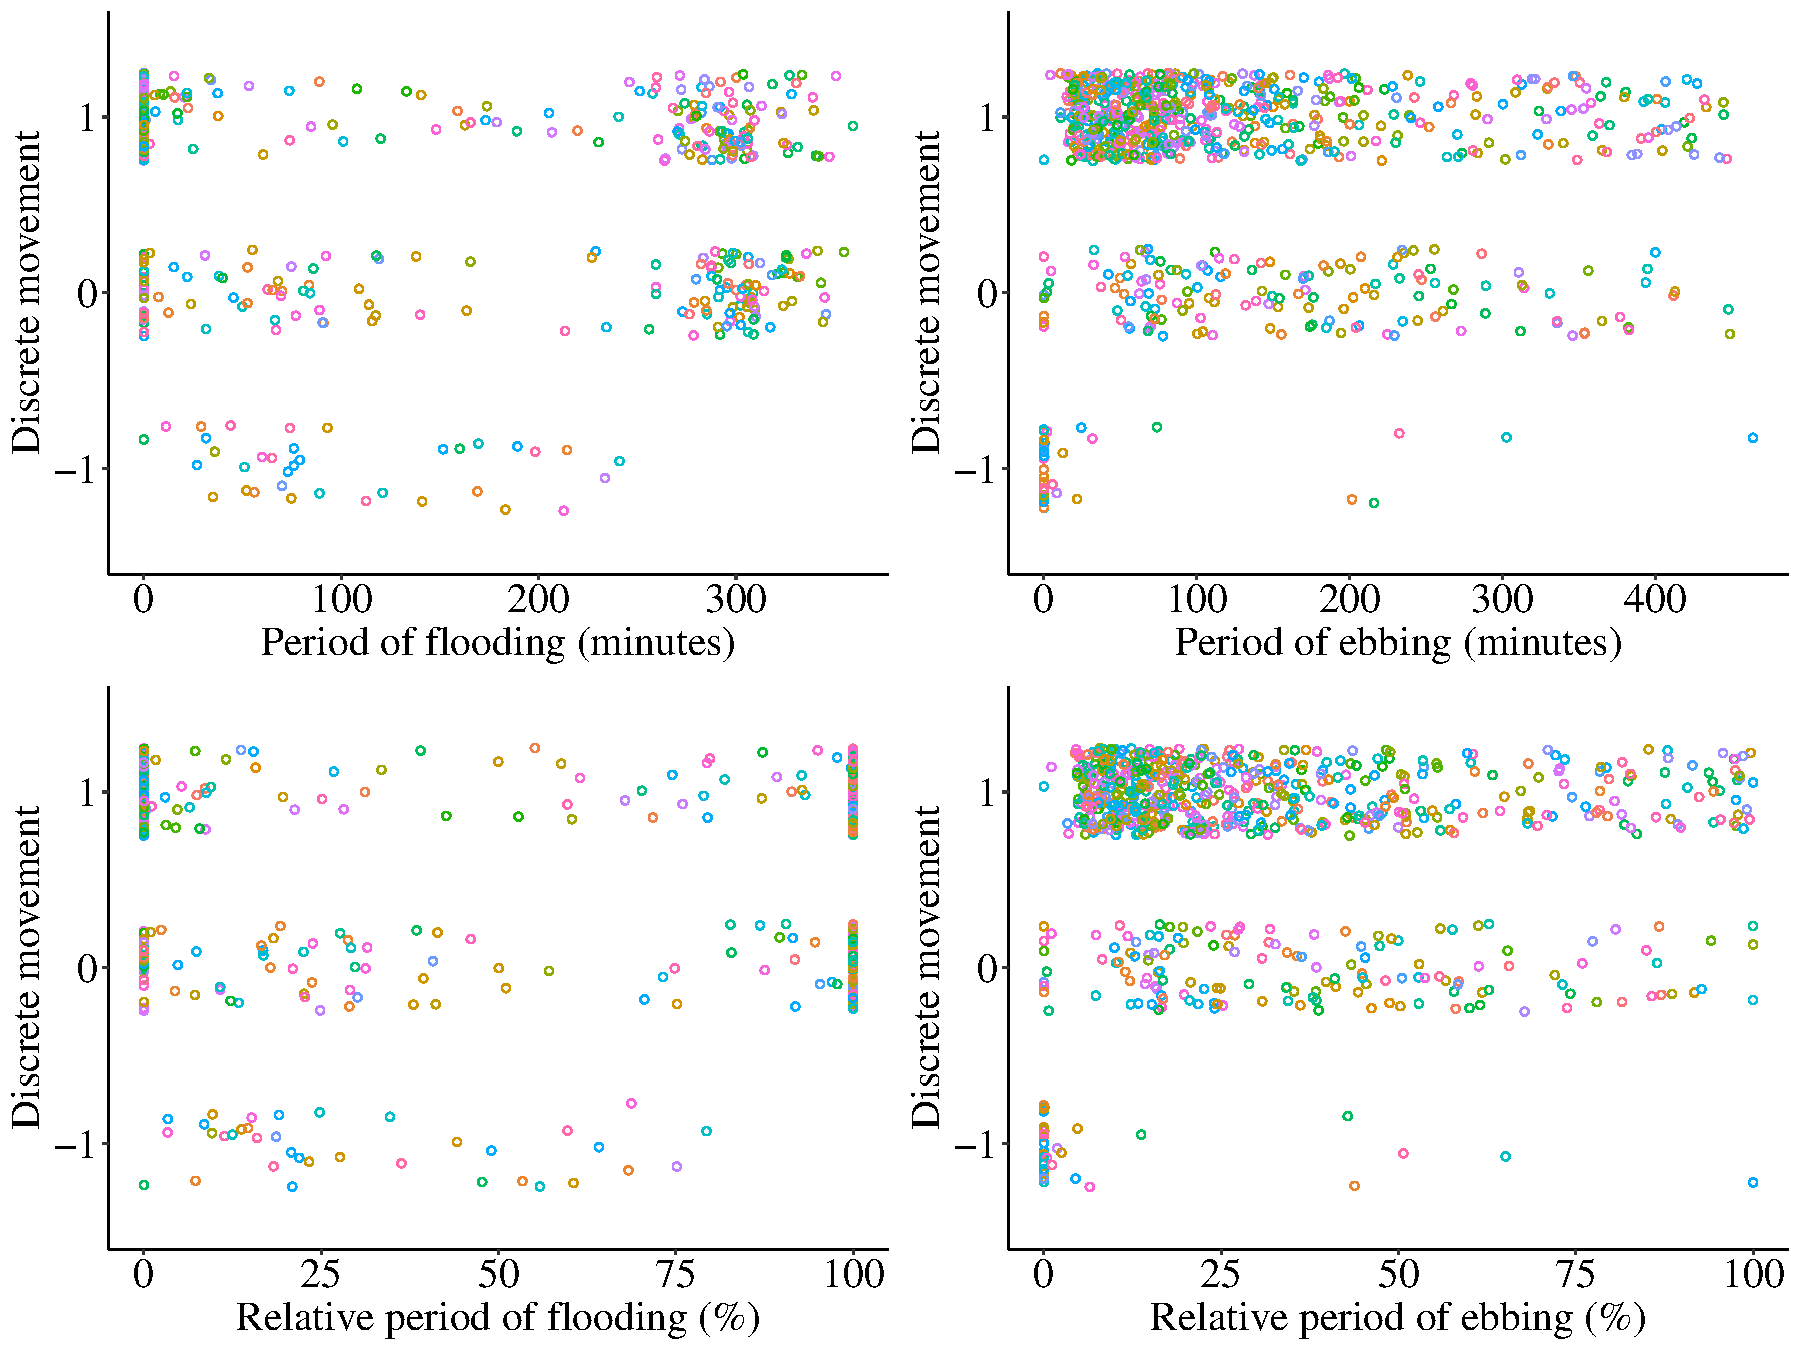
\includegraphics[scale=0.45]{Distance_versus_floodebb.pdf}
  \caption{Graphs of discrete movement. Downstream movement (1); upstream movement (-1); residency (0) versus the relative (\%) and actual (minutes) period of flooding and ebbing. All movement and residency intervals are depicted. Different colors represent different eels.}
  \label{fig:Distance_versus_floodebb}
\end{figure}

\begin{figure}[h!]
  \centering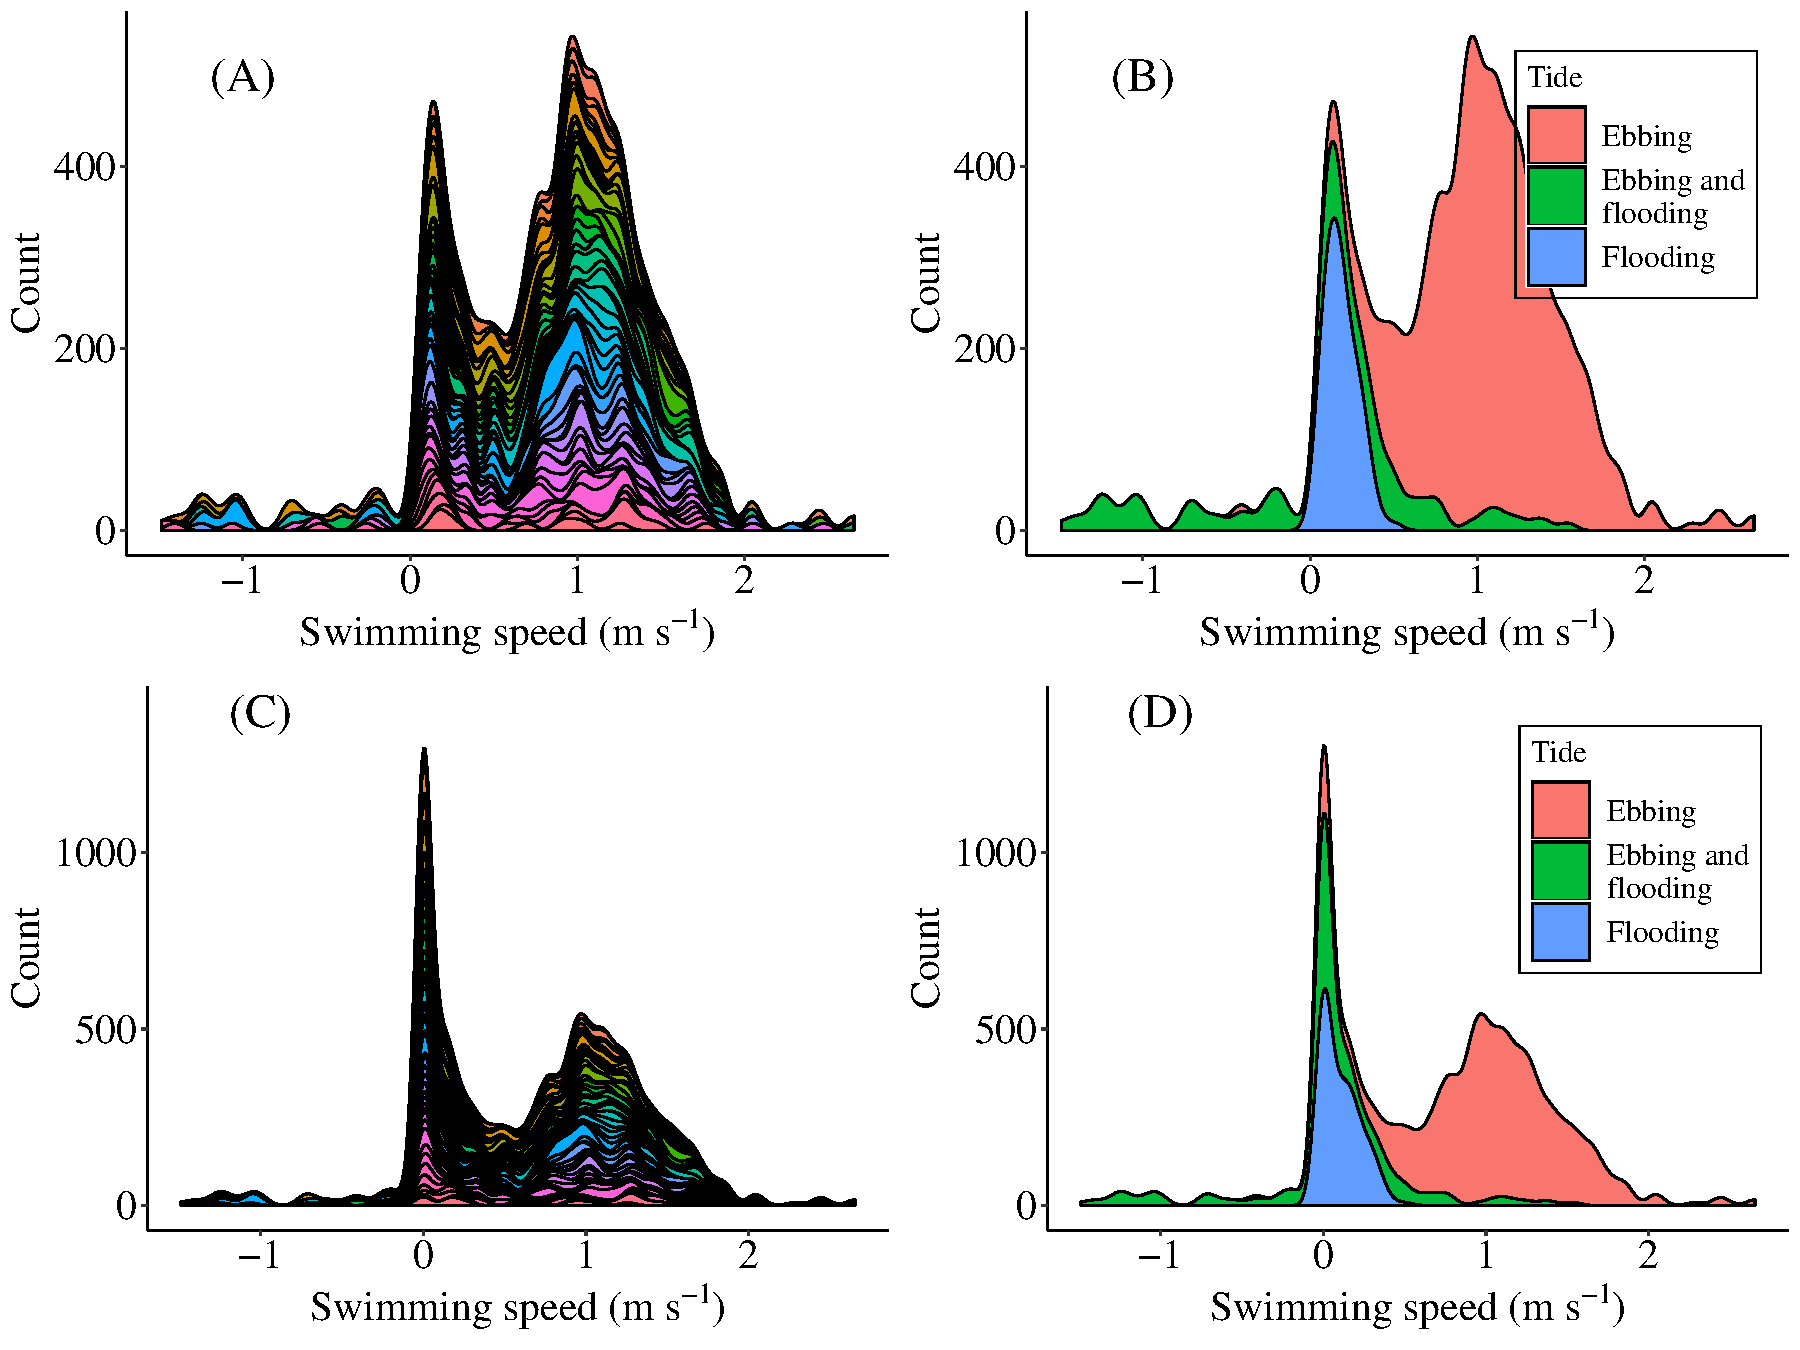
\includegraphics[scale=0.45]{density_count_speed.pdf}
  \caption{Transformed stacked density plots of eel swimming speed (m $s^{-1}$). To determine the count of the stacked density plots, there are several steps involved. First, the x-axis, which represents the swimming speed, is subdivided in swimming-speed intervals with a width of 0.05 m $s^{-1}$. Second, the amount of movement (and residency) intervals for each swimming-speed interval is divided by the swimming-speed interval width. For example, in the swimming-speed interval centering the value 1 m $s^{-1}$, 25 movement intervals were found. Hence, 25 movement intervals divided by a width of 0.05 m $s^{-1}$ yield a count of 500. In A and B the density plots of all movement intervals are given. The different colors in A depict the different eels, while the different colors in B depict whether movement intervals occurred during flooding, ebbing or a combination of both. In C and D the density plots of all residency intervals and movement intervals are given. The different colors in C depict the different eels, while the different colors in D depict whether residency and movement intervals occurred during flooding, ebbing or a combination of both. }
  \label{fig:density_count_speed}
\end{figure}

An exploratory analysis of the data suggests that downstream movement intervals generally took place during ebb tide (Figs \ref{fig:Distance_versus_floodebb} and \ref{Departure_and_arrival}). The normalized duration of flood tide in the downstream movement intervals was either 0 or to a lesser extent 100 \% (Fig. \ref{fig:Distance_versus_floodebb}), suggesting that downstream movement intervals contained either no flooding at all or a full flood cycle. On the other hand, upstream movement intervals typically took place during flood tide (Figs \ref{fig:Distance_versus_floodebb} and \ref{Departure_and_arrival}). Finally, residencies seemed to occur more often during flood tide than during ebb tide (Fig. \ref{fig:Distance_versus_floodebb}). 

Transformed stacked density plots of swimming speed gave additional insights into the distribution of the data (Fig. \ref{fig:density_count_speed}). It is clear from these figures that the bimodal pattern in the data is the result of different tidal conditions rather than of individual differences. Most eels have swimming speeds ranging from 0 to 2 m s$^{-1}$, but swimming speeds from 0 to approximately 0.45 m s$^{-1}$ typically occurred during pure flooding or a combination of flooding and ebbing, while swimming speeds of approximately 0.45 to 2 m s$^{-1}$ typically occurred during pure ebbing events. This suggests that movement intervals with a swimming speed below approximately 0.45 m s$^{-1}$ are likely to contain cryptic residencies, causing a delay in travel time. 

\subsection{Model construction and evaluation}
\label{sect:results:modelconstruct}

\renewcommand{\arraystretch}{1.5}
\begin{table}
\centering
\caption{RMSE values (Eq. \ref{eq:RMSE}) after Monte Carlo cross-validations (10$^{4}$ permutations) for different models and different data subsets.}
\label{tab:RMSE_CV}
\begin{tabular}{l|l|c} 
\toprule
Data                                                                             & Model                                                    & RMSE    \\ 
\midrule
\multirow{5}{*}{\begin{tabular}[c]{@{}l@{}}Original\\data\\set \end{tabular}}    & One-part model                                            & 0.4165  \\
                                                                                 & Two-part model: 0 vs not 0 m s$^{-1}$     & 0.4073  \\
                                                                                 & Selection model: 0 vs not 0 m s$^{-1}$                    & 0.4132  \\
                                                                                 & Three-part model: 0 vs 0 vs 0 m s$^{-1}$                  & 0.4055  \\
                                                                                 & Conditional inference random forests                      & 0.3941  \\ 
\hline
\multirow{5}{*}{\begin{tabular}[c]{@{}l@{}}No\\upstream\\movement \end{tabular}} & \begin{tabular}[c]{@{}l@{}}One-part model\\ \end{tabular} & 0.4051  \\
                                                                                 & Two-part model: 0 vs not 0 m s$^{-1}$                         & 0.3804  \\
                                                                                 & Selection model: 0 vs not 0 m s$^{-1}$                        & 0.5410  \\
                                                                                 & Three-part model: 0 vs 0-0.45 vs 0.45-2.7 m s$^{-1}$      & 0.3653  \\
                                                                                 & Conditional inference random forests                      & 0.3669  \\
\bottomrule
\end{tabular}
\end{table}
\renewcommand{\arraystretch}{1}

\begin{figure}[h!]
  \centering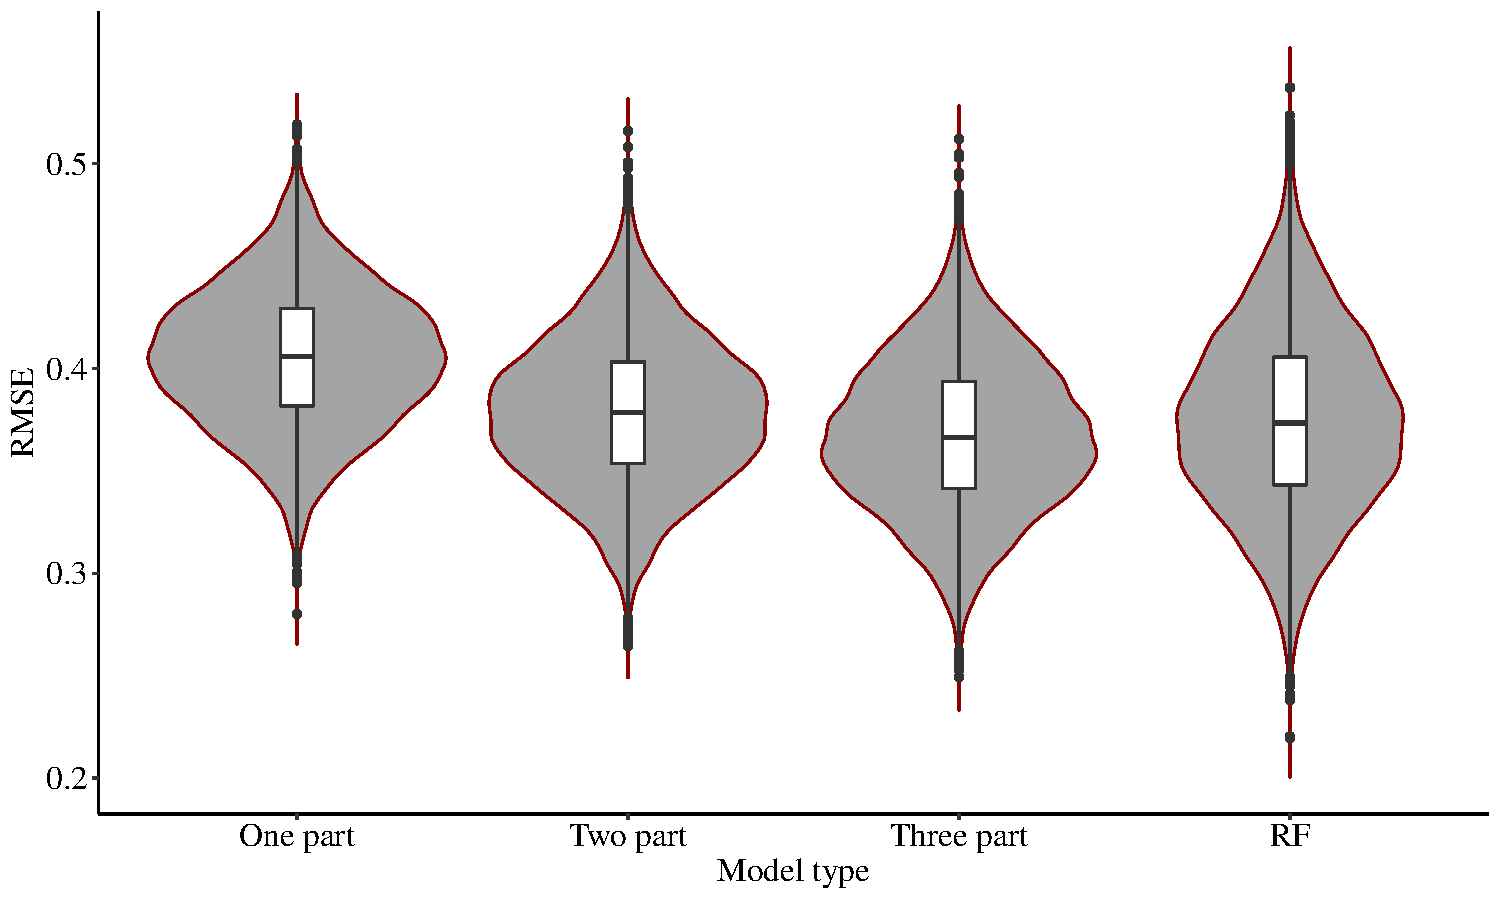
\includegraphics[scale=0.5]{violinRMSE.pdf}
  \caption{Violin plots representing the distribution of RMSE values obtained through cross-validation (n=10$^{4}$) for the different models. RMSE distributions are given for the one-part model, two-part model (0 vs not 0 m s$^{-1}$), three-part model (0 vs 0-0.45 vs 0.45-2.7 m s$^{-1}$) and random forests model (RF). The data set without upstream intervals was used to construct the models.}
  \label{fig:violinRMSE}
\end{figure}

For the original data set, Monte-Carlo cross-validations indicated that the three-part model, which compartmentalized predictions into (1) residencies and (2) downstream and (3) upstream movement, had the highest predictive performance (RMSE = 0.4055), followed by the two-part model (RMSE = 0.4073), which compartmentalized predictions in (1) residencies and (2) movement, the selection model (RMSE = 0.4132) and the one-part model (RMSE = 0.4165) (Table \ref{tab:RMSE_CV}). After transformation of the upstream movement intervals to residency intervals, Monte-Carlo cross-validations indicated that the three-part model, which compartmentalized predictions into classes of (1) 0, (2) 0 to 0.45 and (3) 0.45 to 2.7 m s$^{-1}$, had the highest predictive performance (RMSE = 0.3653) followed by the two-part model (RMSE = 0.3804), which compartmentalized predictions into (1) residencies and (2) movement, one-part model (RMSE = 0.4051) and selection model (RMSE = 0.5410) (Table \ref{tab:RMSE_CV}). Since the three-part model performed best, it was retained for further analysis (Table \ref{tab:Bootstrap_model}). 

\renewcommand{\arraystretch}{1.5}
\begin{table}
\centering
\caption{Parameter estimates, 95\% percentile confidence intervals (CI) and p-values of the one-part, two-part and three-part models obtained using a weighted bootstrap approach (n=10$^{4}$). The models had swimming speed as response and predictors were selected using a bootstrap selection procedure based on backwards elimination and AIC. The considered predictors were flood ratio (\% percentage flood over total period), distance from source (km), moon phase (degree of moon illumination ranging from 0 to 1), tidal phase (ratio of the maximum difference in water level of the concerning day over the median of the maximum difference in water level per day of the entire study period) and day phase (categorical: day, night, dusk or dawn). The data set without upstream intervals was used to construct the models.}
\label{tab:Bootstrap_model}
\scriptsize
\resizebox{1.0\textwidth}{!}{
\begin{tabular}{l|l|l|l|lllll} 
\toprule
\multicolumn{4}{l|}{}                                                                                                                                                                                                                                                          & Intercept       & Flood ratio  & Distance & Moon phase & Tidal phase\\ 
\midrule
\multicolumn{3}{l|}{\multirow{3}{*}{\begin{tabular}[c]{@{}l@{}}One-part \\model \end{tabular}}}                                                                                                                                                                     & Estimate & 0.704           & -0.0124                                                   & 4.94*10$^{-3}$                                         & 0.0885                                                   &                                            \\
\multicolumn{3}{l|}{}                                                                                                                                                                                                                                               & CI       & {[}0.629 0.780]  & {[}-0.0133 -0.0116]                                       & {[}3.57*10$^{-3}$ 6.32*10$^{-3}$]                      & {[}0.0105 0.166]                                         &                                            \\
\multicolumn{3}{l|}{}                                                                                                                                                                                                                                               & p-value  & 0               & 0                                                         & 0                                                      & 0                                                        &                                            \\ 
\hline
\multirow{6}{*}{\begin{tabular}[c]{@{}l@{}}Two-\\part\\model \end{tabular}}    & \multicolumn{2}{l|}{\multirow{3}{*}{\begin{tabular}[c]{@{}l@{}}Binomial\\model \end{tabular}}}                                                                                     & Estimate & 1.45            & -0.0195                                                   &                                        &                                          &                                            \\
                                                                               & \multicolumn{2}{l|}{}                                                                                                                                                              & CI       & {[}1.31 1.60]   & {[}-0.0231 -0.0160]                                        &                                        &                                          &                                            \\
                                                                               & \multicolumn{2}{l|}{}                                                                                                                                                              & p-value  & 0               & 0                                                         &                                        &                                          &                                            \\ 
\cline{2-9}
                                                                               & \multicolumn{2}{l|}{\multirow{3}{*}{\begin{tabular}[c]{@{}l@{}}Linear \\model \end{tabular}}}                                                                                      & Estimate & 0.795           & -0.0137                                                   & 5.16*10$^{-3}$                                         & 0.0915                                                   &                                            \\
                                                                               & \multicolumn{2}{l|}{}                                                                                                                                                              & CI       & {[}0.725 0.866] & {[}-0.0151 -0.0123]                                       & {[}3.90*10$^{-3}$ 6.43*10$^{-3}$]                       & {[}0.0101 0.174]                                         &                                            \\
                                                                               & \multicolumn{2}{l|}{}                                                                                                                                                              & p-value  & 0               & 0                                                         & 0                                                      & 0.00258                                                  &                                            \\ 
\hline
\multirow{12}{*}{\begin{tabular}[c]{@{}l@{}}Three-\\part\\model \end{tabular}} & \multirow{6}{*}{\begin{tabular}[c]{@{}l@{}}Multi-\\nomial\\model  \end{tabular}} & \multirow{3}{*}{\begin{tabular}[c]{@{}l@{}}0-0.45\\vs \\0 m s$^{-1}$ \end{tabular}}    & Estimate & 0.507           & -0.0134                                                   &                                        &                                          &                                            \\
                                                                               &                                                                                                  &                                                                                 & CI       & {[}0.0830 0.973] & {[}-0.0212 -0.00595]                                      &                                        &                                          &                                            \\
                                                                               &                                                                                                  &                                                                                 & p-value  & 0.105           & 8.00*10$^{-4}$                                            &                                        &                                          &                                            \\ 
\cline{3-9}
                                                                               &                                                                                                  & \multirow{3}{*}{\begin{tabular}[c]{@{}l@{}}0.45-2.7 \\vs \\0 m s$^{-1}$ \end{tabular}} & Estimate & 2.96            & -0.0987                                                   &                                        &                                          &                                            \\
                                                                               &                                                                                                  &                                                                                 & CI       & {[}2.57 3.43]   & {[}-0.117 -0.0835]                                        &                                        &                                          &                                            \\
                                                                               &                                                                                                  &                                                                                 & p-value  & 0.126           & 0.00152                                                   &                                        &                                          &                                            \\ 
\cline{2-9}
                                                                               & \multirow{3}{*}{\begin{tabular}[c]{@{}l@{}}Gamma\\model \end{tabular}}                           & \multirow{3}{*}{\begin{tabular}[c]{@{}l@{}}0-0.45\\m s$^{-1}$ \end{tabular}}           & Estimate & -2.2            & -0.00548                                                  &                                        &                                          & 0.870                                                       \\
                                                                               &                                                                                                  &                                                                                 & CI       & {[}-3.31 -1.12] & {[}-0.00893 -0.00204]                                     &                                        &                                          & {[}-0.192 1.94]                                            \\
                                                                               &                                                                                                  &                                                                                 & p-value  & 0.650            & 0.00167                                                   &                                        &                                          & 0.648                                                      \\ 
\cline{2-9}
                                                                               & \multirow{3}{*}{\begin{tabular}[c]{@{}l@{}}Linear\\model \end{tabular}}                          & \multirow{3}{*}{\begin{tabular}[c]{@{}l@{}}0.45-2.7\\m s$^{-1}$ \end{tabular}}         & Estimate & 0.82            & -0.00455                                                  & 7.22*10$^{-3}$                                         & 0.0425                                                   &                                            \\
                                                                               &                                                                                                  &                                                                                 & CI       & {[}0.750 0.889]  & {[}-0.00690 -0.00219]                                      & {[}5.93*10$^{-3}$ 8.53*10$^{-3}$]                      & {[}-0.0436 0.127]                                        &                                            \\
                                                                               &                                                                                                  &                                                                                 & p-value  & 3.00*10$^{-4}$  & 0                                                         & 0                                                      & 0.0011                                                   &                                            \\
\bottomrule
\end{tabular}
}
\end{table}
\renewcommand{\arraystretch}{1}

The results of the multinomial model of the three-part model indicated that the distinction between <0.45 and >0.45 m s$^{-1}$ was significantly better than the distinction between 0 and 0 to 0.45 m s$^{-1}$. The relative risk ratio for a one-percentage increase in the flood ratio was 0.987 for being between 0 and 0.45 m s$^{-1}$ versus 0 m s$^{-1}$ and 0.907 for being between 0.45 and 2.7 m s$^{-1}$ versus 0 m s$^{-1}$. The higher the flood ratio, the higher the probability of an observed residency interval (0 m s$^{-1}$) and the lower the probability of a movement interval with a swimming speed above 0.45 m s$^{-1}$. The probability of a movement interval with a swimming speed below 0.45 m s$^{-1}$ shows an increasing trend with flood ratio similar to the probability of residency intervals until a flood ratio of approximately 40 \%, after which the probability decreases (Fig. \ref{fig:multinomial}). 

\begin{figure}[h!]
  \centering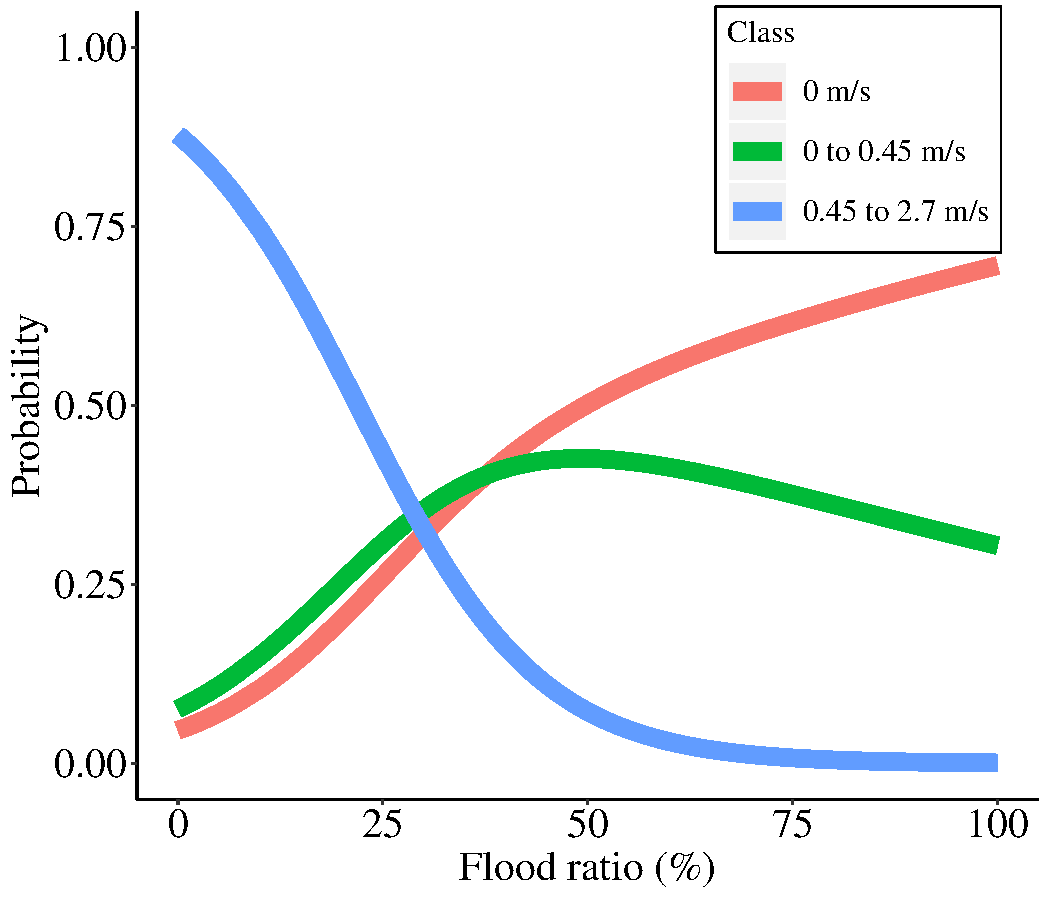
\includegraphics[scale=0.7]{multinomial}
  \caption{Output of the most parsimonious multinomial model with as response the three categories: 0, 0 to 0.45, 0.45 to 2.7 m s$^{-1}$ and as predictor the flood ratio. The probability of each class is given as a function of the flood ratio.}
  \label{fig:multinomial}
\end{figure}

However, distinction between swimming speeds of 0 and 0 to 0.45 m s$^{-1}$ was necessary in order to fit a generalized linear model with gamma distribution through the data. Using a binomial model with contrasts <0.45 and >0.45 m s$^{-1}$ followed by two linear models yielded a lower predictive performance (RMSE = 0.3712) and would have violated model assumptions. The multinomial model on its own provided a relatively low predictive performance (RMSE=0.3940), but addition of a generalized linear model with gamma distribution from 0 to 0.45 m s$^{-1}$ and a linear model from 0.45 to 2.7 m s$^{-1}$ increased the predictive performance with 7.3 \%  (RMSE=0.3653). The gamma model from 0 to 0.45 m s$^{-1}$ indicated a significant negative effect of flood ratio. However, it should be noted that the model fit was relatively poor as using a null model instead decreased the overall predictive performance with only 1.1 \% (RMSE = 0.3693). More benefit was gained from the linear model for the part of 0.45 to 2.7 m s$^{-1}$ as its omission reduced overall predictive performance with 6.7 \% (RMSE = 0.3898). The flood ratio and moon phase had a significantly negative and positive effect on the swimming speed, respectively, but were found to be far less important than the significant positive effect of the distance to source. During ebbing tide, eels closer to the North Sea had relatively higher swimming speeds. Finally, all full model-parts of this three-part model were offered the variable eel ID as fixed factor in the model selection process, but it was only retained in the latter linear model from 0.45 to 2.7 m s$^{-1}$. This suggests that individual differences were important to predict swimming speeds from 0.45 to 2.7 m s$^{-1}$, but not to distinguish between classes (1) 0, (2) 0 to 0.45 and (3) 0.45 to 2.7 m s$^{-1}$ or to predict the swimming speed from 0 to 0.45 m s$^{-1}$.

Similar predictors with reliable parameter estimates were retained in the different models (Table \ref{tab:Bootstrap_model}). For the binomial part of the two-part models only flood ratio was retained, while the one-part models and linear parts of the two-part models retained, in order of decreasing importance, the factors flood ratio, distance to source and moon phase. The variable importance provided by the conditional inference random forests indicated that flood ratio (0.3733) was most important, followed by distance from source (0.0609), moon phase (0.0218), tidal phase (0.0204) and day phase (0.00796). The conditional inference random forests performed better (2.8 \%) than the best statistical model when considering upstream movement intervals, but performed slightly worse (0.4 \%) than the best statistical model when  upstream movement intervals were not considered. 

RMSE values of the one-part and two-part mixed models for the data set without upstream movement intervals were 0.373 and 0.347 respectively. Hence, the two-part mixed model explained patterns in the data 7.0 \% better than the one-part mixed model.

\FloatBarrier

\section{Discussion}

\subsection{Evaluating one-part, two-part and three-part (mixed) models}

Movement decisions have been assessed in depth for a wide range of animals \citep{Berdahl2017SocialFish,Dechmann2017DeterminantsBat,ONeal2018TheDucks}, but the number of studies combining movement decisions with movement intensity, e.g. swimming speed or distance covered, has been limited \citep{Brodersen2008OptimalFish}. Because zero values describe a unique behavioral aspect in movement behavior, i.e. residencies, defining observed zeros and identifying cryptic zeros in telemetry data sets allowed to improve predictive performance and to obtain more detailed ecological insights. The predictive performances of the original three-part and two-part models were higher (between 2.2 and 9.8 \%) than those of the one-part models, suggesting that the conditions that affect the movement decision are not necessarily the same as the conditions that affect the movement intensity. Taking into consideration that both processes might be correlated did not improve predictions as the selection models had a lower predictive performance. This is in concordance with many econometric studies in which accounting for potential dependencies between both parts of the model did not seem to add to the quality of the predictions \citep{Madden2008SampleDrinking,Smith2003OnModels}. 

Although distinguishing between movement and residencies provided clearly better predictions, further distinction between upstream and downstream movement only provided marginally better predictive performances (0.4 \%). This might be because of the limited amount of upstream movement intervals and the limited amount of individuals exhibiting upstream movement, causing only a limited increase in explanatory power in the test set. However, the poor gain in explanatory power of the model may also be the result of the similar conditions in which upstream movement and residencies occurred. Indeed, considering upstream movement as residencies gone wrong, resulted in a 6.6 \% and 2.7 \% increase in performance for the two-part and one-part model respectively. This suggests that some eels are unsuccessful in remaining resident during flooding as they are pushed back, or that they mistake flooding for ebbing when moving along with the current. A final improvement of model performance was apparent from further compartmentalization. Distinction between swimming speeds of (1) 0, (2) 0 to 0.45 and (3) 0.45 to 2.7 m s$^{-1}$ caused predictions of swimming speed to be 9.8 \% better. This model improvement was mainly the result of the contrasting tidal conditions before and after 0.45 m s$^{-1}$, with eels facing or not facing a flooding event respectively. Hence, compartmentalization was successful because it adequately classified observed residencies (0 m s$^{-1}$), cryptic residencies (0 to 0.45 m s$^{-1}$) and movement intervals (0.45 to 2.7 m s$^{-1}$). 

The results of the three-part model suggest that the movement decision depends only on the tides, while the swimming speed is dependent on the tides and the distance from source. The larger the contribution of flood, the more likely a specific time lapse will be a residency interval rather than a movement interval. In addition, eels which migrated during ebb tide and which were already close to the sea, typically had the highest swimming speed. The conditions during which the movement intervals of the first peak of the bimodal pattern (<0.45 m s$^{-1}$) occurred were actually more closely related to those of residency intervals than those of movement intervals of the second peak of the bimodal pattern (>0.45 m s$^{-1}$). Within the observed movement intervals characterized by a swimming speed below 0.45 m s$^{-1}$, cryptic or undetected residencies were invoked by flooding events. During these flooding events, eels had to interrupt their journey, causing lower observed swimming speeds. For swimming speeds above 0.45 m s$^{-1}$, the distance to the North Sea seemed to play a more important role than the tides. In addition, individual variation was significantly more important for swimming speeds above than below 0.45 m s$^{-1}$ and also the movement decision did not show any significant individual variation. This suggests that all eels stay resident during flood, but also that some eels swim faster or slower than others once the decision to continue their migration has been made. The simple position estimates of a single individual would have made it difficult to classify apparent non-movement as either (i) residencies or (ii) movement without net gain in distance covered. However, the ability to quantify individual variation from a large number of tagged individuals provided evidence in favor of the first option. More specifically, as there were clearly faster and slower swimming individuals, the second option would have resulted in meaningful differences between individuals across all parts of the model (i.e. some individuals would be pushed back while others would advance during flood). This was, however, not the case. 

One major advantage of telemetry is its ability to provide data on the level of individuals, and therefore mixed models that account for individual correlation are commonly used \citep{Gillies2006ApplicationAnimals,Hooten2017AnimalData}. Two-part and three-part models can be easily extended to include mixed effects in order to provide a higher explanatory power. In this study, the explanatory power of mixed two-part models was 7.0 \% higher than their one-part equivalents. However, it should be noted that potential dependencies between the elements of random and fixed factors across the different parts were not considered. If correlation between the random effects across the different parts is expected, a joint maximization of the likelihood functions would be required. More research is needed to evaluate the added value of such an approach as its importance is likely to be case-specific. 

Eels have already been shown to exhibit selective tidal stream transport (STST), as they make use of the tides to reach their destination with as little energy expenditure as possible \citep{Barry2016FreshwaterAnguilla,Verhelst2018}. However, by comparing one-part with two-part and three-part models, we illustrated that migrating fish exhibit complex behaviour and that models initially constructed to assess human customer behavior, might also be of use to study other animals \citep{Farewell2017Two-PartData}. 

\subsection{Statistical models versus machine learning}

Statistical models are generally preferred over machine learning when the number of available predictors is limited and the main purpose is to infer ecological knowledge, while the contrary is true if predictive performance is deemed more important than inference. Since researchers often seek to optimize both knowledge and predictions, a mutually exclusive approach should be avoided. In this study we started off with a simple linear regression (i.e. one-part model), then moved further to a two-part model which combined a binomial regression with linear regression, and finally ended up with a three-part model which combined a multinomial model (via neural networks, i.e. machine learning), generalized linear regression with gamma distribution and linear regression. Because each step of the model improvement was supported by ecological knowledge, i.e. being aware that the conditions that cause eels to reside or to move might be different, and methodological considerations, i.e. residencies taking place between gates are not directly observed but do cause a travel delay, the final three-part model remained interpretable. The conditional inference random forests provided similar results, though less informative, and had only slightly higher or lower predictive performances than the developed three-part models. Hence, appreciating the potential complexity of animal behaviour and awareness towards the statistical framework that machine learning algorithms are built upon, will provide researchers with the best machine learning has to offer without compromising the lessons learnt from statistical models. 

\subsection{Recommendations for future studies}

In order for zero values to provide useful information, a good understanding of the meaning of zeros in the data is required. In this study we considered all observed zeros to be true zeros, which is a plausible assumption given the high detection probability of the network and mainly unidirectional movement of migrating eel. In contrast, in case detection probabilities are low, many zero values might actually be false zeros as the result of important design and/or observer errors, and hence the probability of a false zero should be explicitly integrated in the model. Since the detection probability is affected by the network design, transmission intervals and detection range, which in turn is affected by environmental conditions \citep{Reubens2018}, an elaborate addition to the two-part models may be required to deal with high levels of false zeros. In addition, a good understanding of the detection range variability is also necessary to estimate any difference between the observed and actual biological response. For instance, in this study, the observed swimming speed of eel likely differed from the actual swimming speed because of the unaccounted detection range variability. Furthermore, the factors known to affect the detection range, i.e. tides \citep{Mathies2014EnvironmentalArrays}, also seem to be affecting the movement behaviour of eel, introducing not only noise but even a potential bias in the data. Independent range tests at different locations along the estuary and at different moments within the tidal cycle are a necessary addition to quantify the noise and/or bias associated with detection range variability \citep{Kessel2014}. 

It should also be noted that some limitations are inherent to the applied technique of passive telemetry and can only be resolved by additional data collection. For example, when eels are between gates and there seem to be travel delays during flood, apparent from reduced swimming speed, it is difficult to tell whether eels (i) remained stationary near the bottom to preserve energy or (ii) swam against the currents without much gain in distance covered. Although the constructed models indicated that the first option is much more likely than the second, depth profiles and actual swimming speed measurements, obtained through archival tags with depth sensors and accelerometers, would provide more direct estimates of specific animal behavior and would allow to validate the results of this study.  

\section{Conclusion}

In this study we illustrated how accounting for both well-defined and cryptic residencies provides a better insight into the movement behaviour of migrating eel. Two-part and three-part models turned out to be promising tools to deal with zero-inflated telemetry data, underlining the complex behaviour of migrating fish. Nevertheless, a sound assessment of the detection range variability in combination with more fine-scale measurements of environmental variables, is necessary in order to confirm the observed patterns in eel movement and its relationship with environmental variables. Although only data from one species, one telemetry network and one telemetry technique was used, the proposed model framework can be used for study cases with other species, networks and techniques (e.g. passive integrated transponder and radio telemetry). 

%%TC:ignore

\section*{\ackname}

This work was supported by the Flemish branch of the LifeWatch ESFRI observatory. P. Verhelst acknowledges the support of the Flemish Agency for Innovation and
Entrepreneurship (VLAIO), now under the auspices of the National Science Fund FWO, during a large part of this study. R. Baeyens, N. De Maerteleire, S. Franquet, E. Gelaude, T. Lanssens, S. Pieters, K. Robberechts, T. Saerens, R. van der Speld, S. Vermeersch and Y. Verzelen assisted with the data collection. B. Lonneville aided in the creation of the map. This work makes use of data and infrastructure provided by VLIZ and INBO and funded by Research Foundation - Flanders (FWO) as part of the Belgian contribution to LifeWatch. We would also like to thank the Royal Belgian Institute of Natural Sciences, Operational Directorate Natural Environment (RHIB Tuimelaar) for infrastructure provision and Rijkswaterstaat (The Netherlands) for their cooperation and the permission to use their marine buoys. This research has benefitted from a statistical consult with Ghent University FIRE (Fostering Innovative Research based on Evidence)

\section*{\autcont}

S.B. conceived the ideas and designed methodology, analyzed the data and led the writing of the manuscript; P.V., J.R. and S.B. collected the data; All authors contributed critically to the drafts and gave final approval for publication.

\section*{\datacc}

The R code, subset of data and documentation are available on Mendeley Data: \url{http://dx.doi.org/10.17632/vtrxw2m9wp.1}

\newpage

\section{References}

\bibliographystyle{elsarticle-harv-noURL.bst}
\bibliography{references.bib}

\newpage

\appendix

\section{Tagging procedure}
\label{Taggingprocedure}

The following description is adopted from \citet{Verhelst2018}. 100 Eels were caught and tagged at the tidal weir in Merelbeke in the Zeeschelde during late summer and autumn (September–November) of three consecutive years (2015 till 2017) using double fyke nets. After periods of heavy rain, water flows over the sluices allowing eels to swim over the sluices. Placing the fyke nets behind the sluices and during periods of heavy rain, allowed to coordinate capture events and improve the chance of capturing eel. Several morphometric features were measured in order to determine the eel maturation stage \citep{Durif2005}: Total length (TL, to the nearest mm), body weight (W, to the nearest g), the vertical and horizontal eye diameter (EDv and EDh respectively, to the nearest 0.01 mm) and the length of the pectoral fin (FL, to the nearest 0.01 mm) (Table \ref{eel_morph}). Only females were tagged, since males are smaller than the minimum size handled in this study (< 450 mm \citep{Durif2005}). Eels of three different maturation stages were tagged: premigrant (F3, n = 51) and the two migrant stages F4 and F5 (n = 21 and n = 28, respectively). The eels were tagged with V13 coded acoustic transmitters (13 x 36 mm, weight in air 11 g, frequency 69 kHz, ping frequency: 60–100 s; estimated battery life: 1021-1219 days (battery life time depended on specific transmitter settings), (Table \ref{settingsTaggedEels})) from VEMCO Ltd (Canada). After anaesthetizing them with 0.3 ml/L clove oil, tags were implanted with permanent monofilament \citep{Thorstad2013b}. Eels recovered in a quarantine reservoir for approximately one hour and were subsequently released at the nearest receiver. 

\setcounter{table}{0} \renewcommand{\thetable}{A.\arabic{table}}

\renewcommand{\arraystretch}{1.5}
\begin{table}[]
\centering
\scriptsize
\caption{Number of all tagged female eels per stage with the different morphometrics: total length (TL), body weight (BW), horizontal and vertical eye diameters (EDh and EDv, respectively) and pectoral fin length (FL). Mean, standard deviation and range (between brackets) are indicated (Adopted from \citet{Verhelst2018}).}
\label{eel_morph}
\begin{tabular}{lllllll}
\toprule
Stage & Number & TL (mm)                                                         & BW (g)                                                             & EDh (mm)                                                               & EDv (mm)                                                              & FL (mm)                                                                 \\ \midrule
F3  & 51     & \begin{tabular}[c]{@{}l@{}}$702 \pm $57 \\ (568 - 835)\end{tabular} & \begin{tabular}[c]{@{}l@{}}$674 \pm $165 \\ (324 - 1106)\end{tabular}  & \begin{tabular}[c]{@{}l@{}}$8.08 \pm $0.57 \\ (6.77 - 9.08)\end{tabular}   & \begin{tabular}[c]{@{}l@{}}$7.55 \pm $0.60 \\ (6.20 - 9.70)\end{tabular}  & \begin{tabular}[c]{@{}l@{}}$32.92 \pm $3.29 \\ (26.76 - 40.32)\end{tabular} \\ 
F4   & 21     & \begin{tabular}[c]{@{}l@{}}$810 \pm $57 \\ (707 - 932)\end{tabular} & \begin{tabular}[c]{@{}l@{}}$1162 \pm $217 \\ (771 - 1830)\end{tabular} & \begin{tabular}[c]{@{}l@{}}$10.41 \pm $0.92 \\ (9.13 - 12.49)\end{tabular} & \begin{tabular}[c]{@{}l@{}}$9.66 \pm $0.78 \\ (8.60 - 11.86)\end{tabular} & \begin{tabular}[c]{@{}l@{}}$40.86 \pm $4.32 \\ (30.84 - 48.18)\end{tabular} \\ 
F5    & 28     & \begin{tabular}[c]{@{}l@{}}$662 \pm $56 \\ (575 - 775)\end{tabular} & \begin{tabular}[c]{@{}l@{}}$585 \pm $144 \\ (417 - 912)\end{tabular}   & \begin{tabular}[c]{@{}l@{}}$9.33 \pm $0.80 \\ (8.14 - 11.18)\end{tabular}  & \begin{tabular}[c]{@{}l@{}}$8.80 \pm $0.79 \\ (7.62 - 10.39)\end{tabular} & \begin{tabular}[c]{@{}l@{}}$34.41 \pm $3.68 \\ (28.97 - 45.37)\end{tabular} \\ \bottomrule
\end{tabular}
\end{table}
\renewcommand{\arraystretch}{1}

\renewcommand{\arraystretch}{1.25}
\begin{table}[]
\centering
\scriptsize
\caption{The number and settings of the transmitters of all tagged eels per step: power output (PO; L = low power output, H = high power output), ping frequency (s) and the time duration (days) per step as well as the total battery life time (days). (Adopted from \citet{Verhelst2018})}
\label{settingsTaggedEels}
\begin{tabular}{l|lll|lll|l} 
\toprule
\multirow{2}{*}{\begin{tabular}[l]{@{}l@{}}Number \\ of \\ transmitters \end{tabular}} & \multicolumn{3}{c|}{Step 1}                                                                                                          & \multicolumn{3}{c|}{Step 2}                                                                                                          & \multirow{2}{*}{\begin{tabular}[l]{@{}l@{}}Battery \\ life \\ (days) \end{tabular}}  \\
                                                                                       & PO & \begin{tabular}[l]{@{}l@{}}Ping \\ frequency  (s) \end{tabular} & \begin{tabular}[l]{@{}l@{}}Duration \\ (days) \end{tabular} & PO & \begin{tabular}[l]{@{}l@{}}Ping \\ frequency (s) \end{tabular} & \begin{tabular}[l]{@{}l@{}}Duration \\ (days) \end{tabular} &                                                                                      \\ 
\midrule
20                                                                                     & L  & 60 - 100                                                          & 1216                                                        & NA & NA                                                                & NA                                                          & 1216                                                                                 \\
40                                                                                     & H  & 60 - 100                                                          & 120                                                         & L  & 60 - 100                                                          & 901                                                         & 1021                                                                                 \\
40                                                                                     & H  & 60 - 100                                                          & 120                                                         & L  & 60 - 100                                                          & 902                                                         & 1022                                                                                 \\
\bottomrule
\end{tabular}
\end{table}
\renewcommand{\arraystretch}{1}

\section{Telemetry network}
\label{Telemetry_network}
\setcounter{table}{0} \renewcommand{\thetable}{B.\arabic{table}}

\renewcommand{\arraystretch}{1.25}
\begin{table}
\centering
\scriptsize
\caption{List of gates, with distance from Ghent (km), deployment date, number of included receivers, period of receiver inactivity and detection probability. Receiver inactivity represents the period during which one receiver of the gate was inactive. Adapted from \cite{Bruneel2020QuantifyingSystems}.}
\label{gate_list}
\begin{tabular}{c|ccccc} 
\toprule
\begin{tabular}[c]{@{}c@{}}gate\\name \end{tabular} & \begin{tabular}[c]{@{}c@{}}Distance\\(km) \end{tabular} & \begin{tabular}[c]{@{}c@{}}Deployment\\date \end{tabular} & \begin{tabular}[c]{@{}c@{}}Number\\of receivers \end{tabular} & Receiver inactivity          & \begin{tabular}[c]{@{}c@{}}Det. prob. \\(\%)\end{tabular}  \\ 
\midrule
s1                                                  & 0.0                                                     & 31/03/2015                                                & 1                                                       &                         & 100.0                                                                   \\ 
s2                                                  & 6.6                                                     & 20/03/2016                                                & 1                                                       &                         & 100.0                                                                   \\ 
s3                                                  & 12.1                                                    & 20/03/2016                                                & 1                                                       &                         & 97.1                                                                    \\ 
s4                                                  & 16.8                                                    & 20/04/2015                                                & 1                                                       &                         & 97.4                                                                    \\ 
s5                                                  & 26.7                                                    & 31/03/2015                                                & 1                                                       &                         & 99.1                                                                    \\ 
s6                                                  & 30.6                                                    & 2/04/2015                                                 & 1                                                       &                         & 98.7                                                                    \\ 
s7                                                  & 33.0                                                    & 24/03/2016                                                & 1                                                       & 17/10/2017 - 24/11/2017 & 96.7                                                                    \\ 
s8                                                  & 39.3                                                    & 24/03/2016                                                & 1                                                       &                         & 81.6                                                                    \\ 
s9                                                  & 40.8                                                    & 20/04/2015                                                & 1                                                       &                         & 99.9                                                                    \\ 
s10                                                 & 44.1                                                    & 20/04/2015                                                & 1                                                       &                         & 99.3                                                                    \\ 
s11                                                 & 46.5                                                    & 27/04/2015                                                & 1                                                       &                         & 100.0                                                                   \\ 
s12                                                 & 49.0                                                    & 2/04/2015                                                 & 1                                                       &                         & 98.4                                                                    \\ 
s13                                                 & 53.8                                                    & 2/04/2015                                                 & 1                                                       &                         & 93.2                                                                    \\ 
s14                                                 & 55.6                                                    & 2/04/2015                                                 & 1                                                       &                         & 100.0                                                                   \\ 
s15                                                 & 63.3                                                    & 2/04/2015                                                 & 2                                                       &                         & 100.0                                                            \\ 
s16                                                 & 68.6                                                    & 2/04/2015                                                 & 2                                                       &                         & 100.0                                                            \\ 
s17                                                 & 75.8                                                    & 30/09/2015                                                & 3                                                       &                         & 100.0                                                               \\ 
s18                                                 & 88.2                                                    & 3/09/2015                                                 & 2                                                       &                         & 77.8                                                             \\ 
ws1                                                 & 112.8                                                   & 22/09/2015                                                & 6                                                       &                         & 91.3                                                             \\ 
                                         
\bottomrule
\end{tabular}
\end{table}
\renewcommand{\arraystretch}{1}

\section{Figures}
\setcounter{figure}{0} \renewcommand{\thetable}{C.\arabic{table}}
\begin{figure}[h!]
  \centering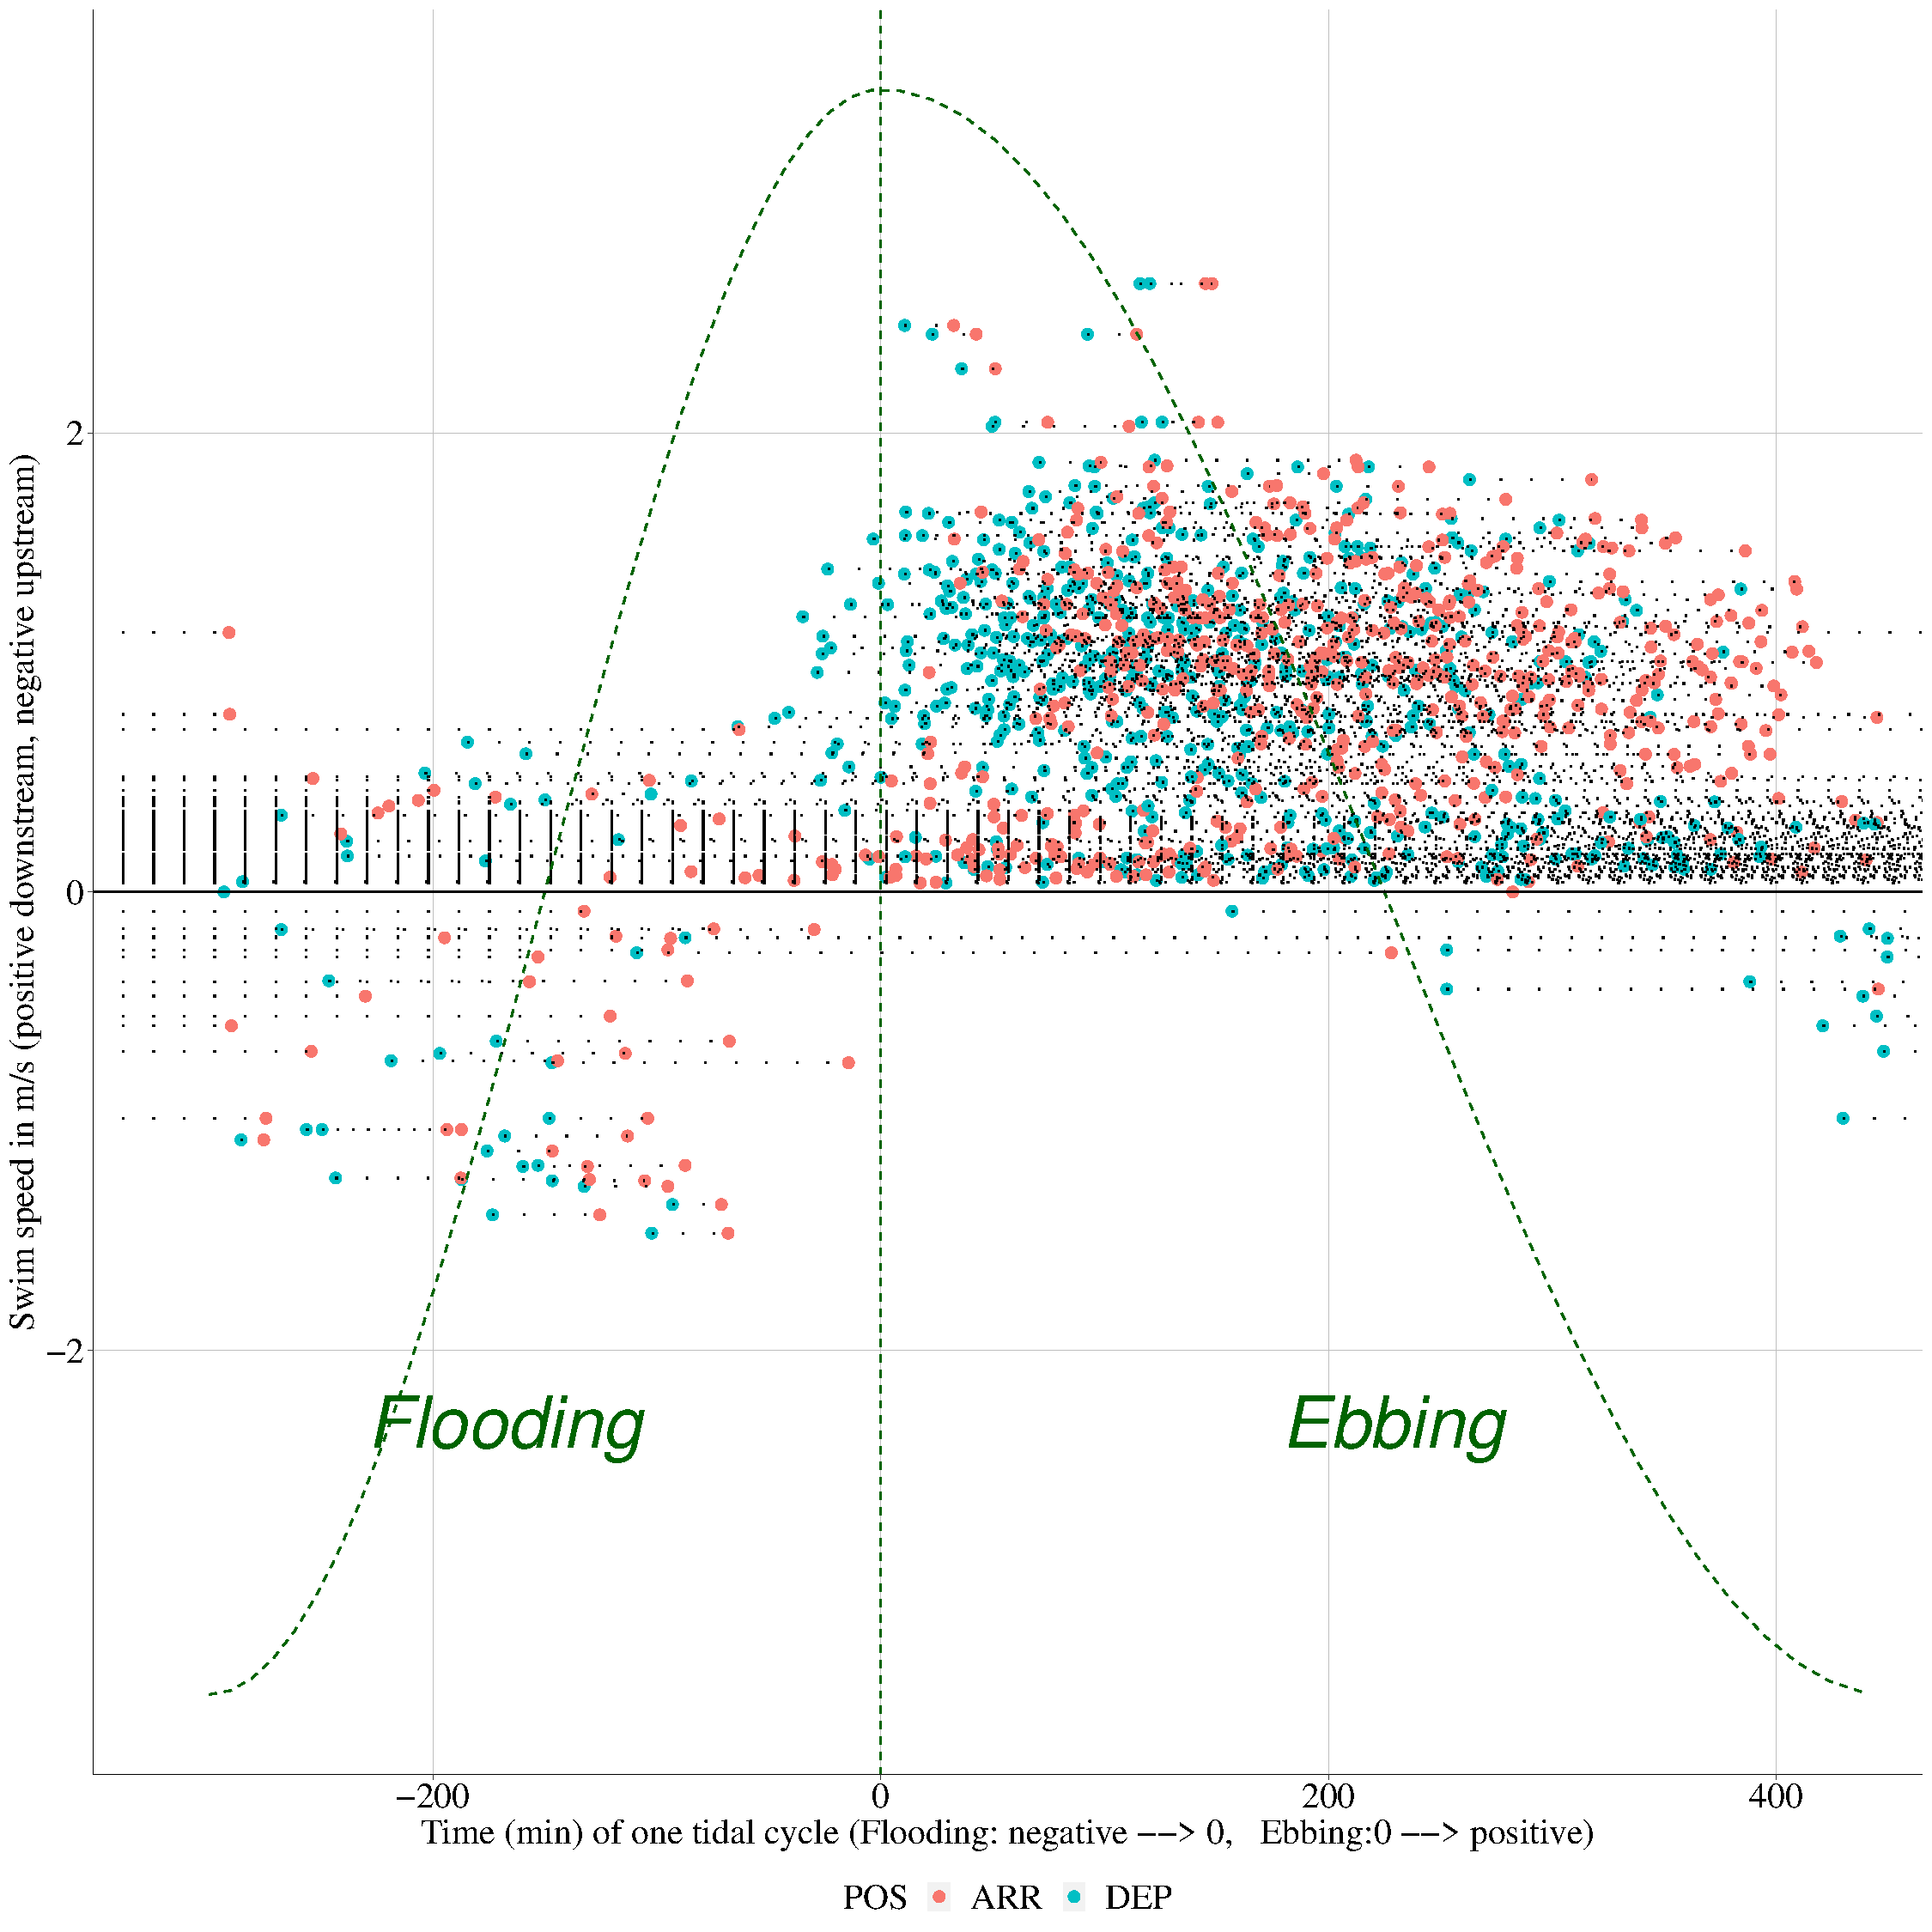
\includegraphics[scale=0.35]{Departure_and_arrival.pdf}
  \caption{Movement intervals of all tagged eels depicted by the departure (DEP) from a receiver and arrival (ARR) at another receiver. The swimming speed (m s$^{-1}$) during a movement interval is given in function of the moment within the tidal cycle. In the ZS, the period of ebbing is larger than the period of flooding, with differences being most pronounced upstream. However, for visualization purposes the average period of flooding (300 minutes) and period of ebbing (450 minutes) of the city of Dendermonde (in the center of the ZS) were used to rescale the TMIs \citep{Levy2014HetGetijkarakteristieken}
  }
  \label{Departure_and_arrival}
\end{figure}


%%TC:endignore

\end{document}
